% SPAR Midterm Report Template
% Compatible with arXiv (TeX Live 2023+, pdflatex)
%
% To compile: latexmk -pdf report.tex
% Or use the build scripts: build report.tex

\documentclass[midterm]{sparreport}

\title{Context-Induced Belief Geometry in Large Language Models}

\author{%
  \begin{tabular}{@{}c@{\hspace{3em}}c@{\hspace{3em}}c@{\hspace{3em}}c@{}}
    \textbf{Dani Balcells} & \textbf{Chirag Rastogi} & \textbf{Andrew Lee} & \textbf{Xavier Poncini} \\
    \texttt{dani@example.com} & \texttt{chirag@example.com} & \texttt{andrew@example.com} & \texttt{xavier@example.com} \\[0.2em]
    \small\textit{SPAR Mentee} & \small\textit{SPAR Mentee} & \small\textit{SPAR Mentee} & \small\textit{Supervisor} \\
    & & & \small\textit{Simplex}
  \end{tabular}%
}

\sparround{Spring 2026}

\begin{document}

\maketitle

% ============================================================================
% ABSTRACT (100-200 words)
% ============================================================================
\begin{abstract}
Recent work has established that toy transformers trained on emission data from hidden Markov models (HMMs) linearly encode the current belief state---the posterior distribution over hidden states---in their residual stream~\cite{shai2024}. In this work, we investigate whether this phenomenon arises in-context in a production-scale language model without any additional fine-tuning. Using Llama-3.2-3B prompted with sequences from the Mess3 process, we find that the model reaches near-Bayesian-optimal next-token predictions after roughly 23 tokens, and that linear probes trained on residual stream activations recover the belief state with $R^2 > 0.998$ at mid-early layers. We also present preliminary evidence that the belief state remains linearly decodable even for processes where the mapping from belief states to output probabilities is non-injective, suggesting the model tracks genuine latent structure rather than merely compressing its output distribution. Beyond these correlational findings, we show that the representations are causally relevant: both activation patching and activation steering shift the model's output distribution in the direction of a target belief state. Tuned Lens analysis further reveals that later layers yield sharper per-layer predictions despite exhibiting weaker linear belief-state encoding, posing an open question about how the model routes belief-relevant computation to its output. Future work will study the mechanisms by which the model in-context learns the belief geometry and routes it to its output.
\end{abstract}

\keywords{in-context learning \and hidden Markov models \and belief states \and mechanistic interpretability \and linear probing}

% ============================================================================
% INTRODUCTION
% ============================================================================
\section{Introduction}

A central question about large language models is whether they merely learn surface-level statistical regularities or whether they develop structured internal models of the processes that generate their inputs. Hidden Markov models (HMMs) offer a controlled setting in which to test this: an optimal predictor of HMM-generated sequences must maintain a \emph{belief state}---the posterior distribution over hidden states given the observed history---whereas a model that merely compresses token co-occurrence statistics need not. Shai et al.~\cite{shai2024} showed that toy transformers trained on HMM emission data do in fact linearly encode this Bayesian-optimal belief state geometry in their residual stream. Whether the same holds for large, general-purpose language models processing text in context remains an open question.


Park et al.~\cite{park2025} provided complementary evidence that LLMs prompted with random walks on a fixed graph reorganize their internal activations to track the graph structure rather than the surface token identities. We build on both lines of work by asking whether large language models, when prompted with sequences from an HMM, develop internal representations of the underlying belief state geometry purely in context.

This project investigates four related questions: (1) Can Llama-3.2-3B, prompted with a long sequence from an HMM, approach Bayesian-optimal predictions in context? (2) If so, is the current belief state represented approximately linearly in the residual stream? (3) If so, is this representation used causally, in the sense that modifying it shifts the model's output distribution in a predictable way? (4) How does this representation emerge across layers and context positions, and how is it used to determine output token probabilities?

Developing a principled, theoretically-grounded understanding of the computational structures that arise in large language models during pretraining is of broad relevance to AI safety. Without a clear account of the underlying structures that LLMs build and how those structures relate to their training data and behavior, it is difficult to interpret or trust these models at scale. Establishing what representations LLMs form, how those representations are constructed from context, and how they influence model outputs contributes to the rigorous understanding of LLM behavior that is necessary for anticipating failure modes, understanding what these models have learned, and informing safety-relevant interventions.

% ============================================================================
% METHODOLOGY
% ============================================================================
\section{Methodology}

\subsection{Experimental setup}

We use Llama-3.2-3B~\cite{llama32}, a 28-layer base model with no instruction tuning, to avoid interference from fine-tuning objectives. Activations are extracted via TransformerLens at the output of each residual stream layer.

As the generative process we use Mess3, a three-state HMM over tokens $\{A, B, C\}$ with parameters $x = 0.05$ and $\alpha = 0.9$. The belief state at each sequence position is the posterior distribution over the three hidden states $\mathbf{b}_t = (b_t^{(1)}, b_t^{(2)}, b_t^{(3)})$, which lies on the 2-simplex $\Delta^2 = \{\mathbf{b} \in \mathbb{R}^3 : b^{(i)} \geq 0,\, \sum_i b^{(i)} = 1\}$. Sequences of up to 5,000 tokens are generated per run. Figure~\ref{fig:optimal_belief_simplex} shows the resulting belief geometry: as the observer updates its posterior given each new token, the belief state traces out a characteristic three-pronged structure on the simplex, with high-density clusters near each vertex corresponding to high certainty about the current hidden state.

\begin{figure}[htbp]
  \centering
  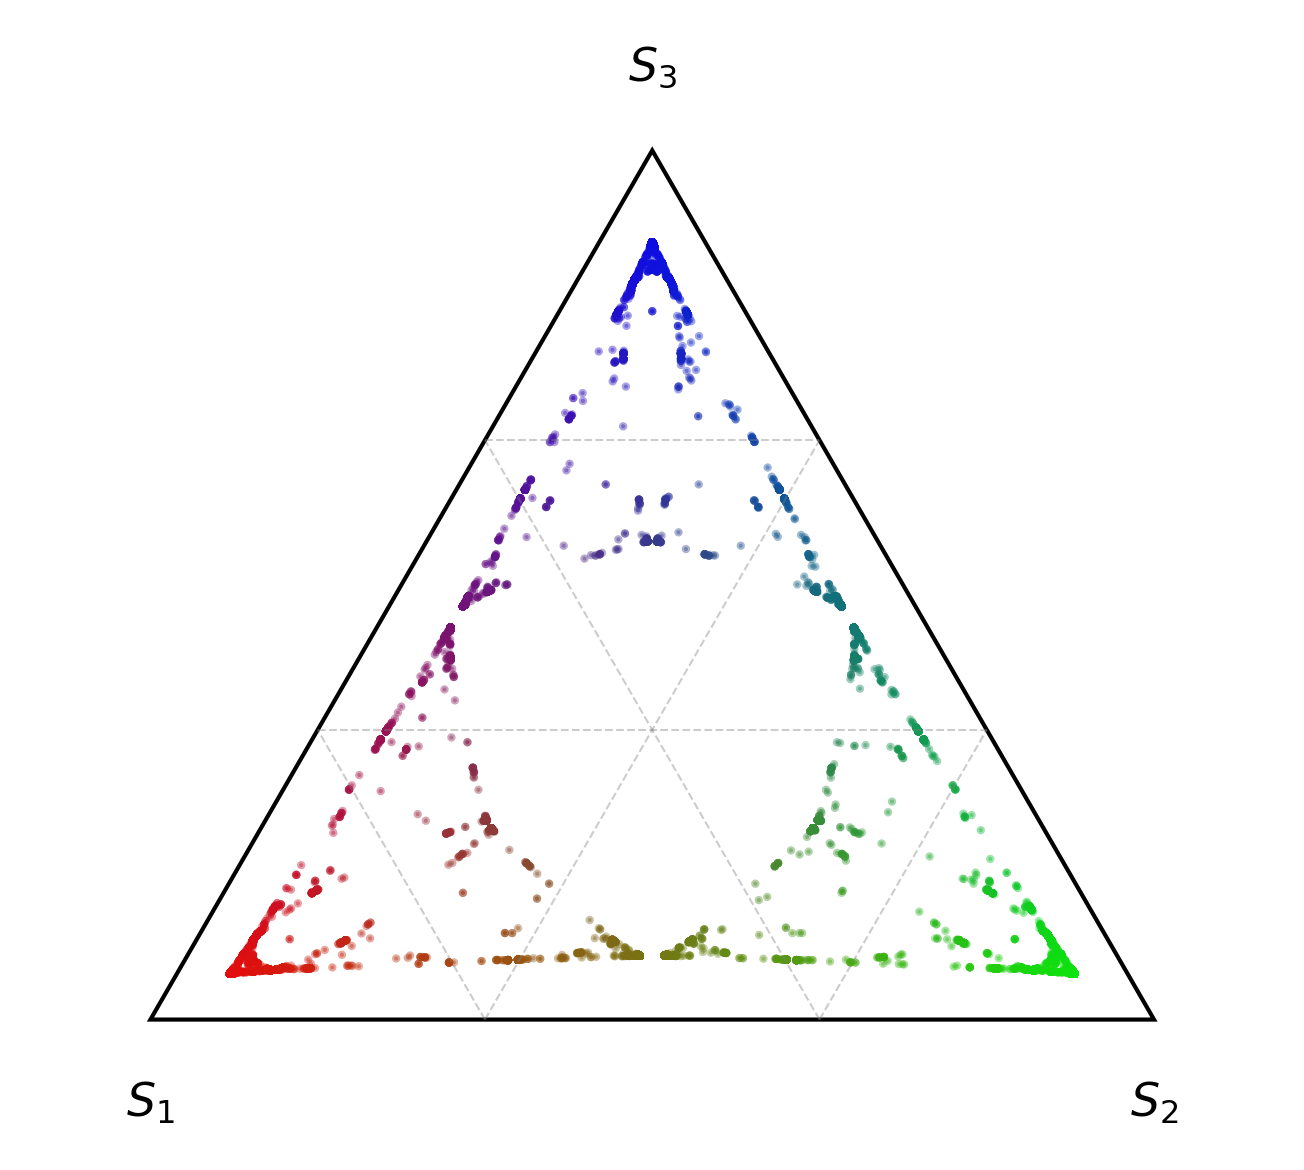
\includegraphics[width=0.45\textwidth]{figures/optimal_belief_simplex.png}
  \caption{Bayesian-optimal belief states pooled across ten 5{,}000-token Mess3 sequences, plotted on the 2-simplex. Each point is one belief state $\mathbf{b}_t$, colored by its value (RGB = $(b_t^{(1)}, b_t^{(2)}, b_t^{(3)})$). The three clusters near the vertices reflect periods of high certainty about the hidden state; the self-similar branching structure between them is characteristic of the fractal belief geometry induced by the HMM.}
  \label{fig:optimal_belief_simplex}
\end{figure}

\subsection{In-context HMM prediction}

\paragraph{Interfacing HMM tokens with the LLM.}
The model's tokenizer does not treat bare single characters and space-prefixed characters identically: the first token in a sequence is encoded as a bare character (e.g.\ \texttt{A}), while all subsequent tokens are encoded as space-prefixed characters (\texttt{{\char`\ }A}, \texttt{{\char`\ }B}, \texttt{{\char`\ }C}), each of which maps to a single entry in the model's vocabulary. At each sequence position $t \geq 1$, we extract the model's logits over the full vocabulary and retain only the three entries corresponding to \texttt{{\char`\ }A}, \texttt{{\char`\ }B}, and \texttt{{\char`\ }C}. The remaining probability mass---assigned to all other vocabulary entries---constitutes a ``junk'' probability that the model places on tokens outside the HMM alphabet.

\paragraph{KL divergence and junk mass.}
To assess whether the model learns to predict Mess3 sequences in context, we measure the KL divergence between the Bayesian-optimal next-token distribution $\mathbf{p}$ and the model's output distribution $\mathbf{q}$ at each position:
\[
  D_{\mathrm{KL}}(\mathbf{p} \,\|\, \mathbf{q})
  = \sum_{k \in \{A,B,C\}} p_k \log \frac{p_k}{q_k}\,.
\]
Because the optimal distribution assigns zero probability to tokens outside $\{A,B,C\}$, the junk term $p_{\text{junk}} \log(p_{\text{junk}} / q_{\text{junk}})$ vanishes and the KL can be computed using only the three HMM token probabilities without renormalization. Note, however, that junk mass still affects the divergence indirectly: probability assigned to non-HMM tokens reduces $q_A + q_B + q_C$ below~1, increasing the KL.

\paragraph{Convergence criterion.}
We define a convergence threshold at 2\% of the maximum KL, smoothed over a 5-token window with a minimum position of 20, and record the token position at which this is first crossed.

\subsection{Linear decodability of belief states}
\label{sec:linear_decodability}

\paragraph{Mess3.}
We extract residual stream activations at each layer and train linear probes (ordinary least squares) to predict the three-dimensional belief state vector from activations. Probes are trained pooled across multiple sequences: 10 training sequences and 5 held-out evaluation sequences, each 5,000 tokens long. We report mean squared error (MSE) and the coefficient of determination $R^2$, evaluated on the held-out sequences.

We also train a paired encoder-decoder: the encoder is a linear map from activations to a learned latent space, and the decoder maps from that latent space back to token probabilities. This gives a complementary measure of how much information relevant to the model's output is mediated through a low-dimensional linear subspace of the residual stream.

\paragraph{Cross-sequence consistency.}
To assess whether different sequences induce similar belief-state representations, we also train separate probes on individual sequences and compare them pairwise. For each layer, we compute the cosine similarity between per-sequence probe weight matrices, the first principal angle $\theta_1$ between the column spaces they span, and the cross-MSE ratio (the MSE when one sequence's probe is applied to another sequence's activations, divided by the self-evaluation MSE). We also compare the pooled probe to each per-sequence probe using the same metrics.

\paragraph{Fern and Leopard.}
A concern with Mess3 is that the emission matrix defines a linear map from the belief state to the output token distribution. This means that a high-quality linear probe could in principle reflect a linear encoding of the model's current output probabilities rather than the belief state proper. In that case, the representation would not require any latent-state tracking beyond what is needed to produce the current output.

The Fern process addresses this ambiguity. It has two output tokens and three hidden states, with an emission matrix that does not admit a left inverse, so the output distribution does not uniquely determine the belief state. Fern is parameterized by a single parameter $x \in [0, 1]$ that controls the coupling between states 1 and 2: the transition matrices interpolate between symmetric ($x = 0$) and maximally asymmetric ($x = 1$) configurations. We test $x \in \{0.4, 0.63\}$. If the model still encodes a three-dimensional belief state geometry for Fern, this provides stronger evidence that it tracks latent states rather than simply compressing its output distribution.

We additionally test the Leopard process, another 3-state, 2-token HMM parameterized by $x \in [0, 1]$, with a sparser, quasi-deterministic transition structure (many zero entries). Leopard tests whether the model can track belief states for processes with sharply different mixing properties. We test $x \in \{0.15, 0.5\}$.

\paragraph{Belief-state sweep.}
To systematically assess how HMM structure affects belief-state encoding, we run a sweep across all three process families (Mess3, Fern, Leopard) and multiple parameterizations, totaling 8 configurations. For each configuration, we generate 50 sequences of length 1000 tokens (20 train, 30 test), extract residual stream activations at all 28 layers, train linear probes (ridge regression) to decode the 3D belief-state vector, and visualize the activation geometry via 2D PCA projections colored by belief state.

\paragraph{Tuned lens sweep.}
For each configuration in the belief-state sweep, we train two types of per-layer affine translators (tuned lenses):
\begin{itemize}
  \item \textbf{Model-target:} Trained to minimize $D_{\mathrm{KL}}(\mathbf{p}_{\mathrm{final}} \,\|\, \mathrm{softmax}(T_l(\mathbf{h}_l) \cdot W_{\mathrm{concept}} + \mathbf{b}_{\mathrm{concept}}))$, where $T_l$ is an identity-initialized affine transformation and $\mathbf{p}_{\mathrm{final}}$ is the model's final-layer output distribution over concept tokens.
  \item \textbf{HMM-target:} Trained with the same architecture but targeting the HMM's observation probabilities (ground-truth next-token distribution given the belief state).
\end{itemize}
This yields four KL divergence metrics per layer: $D_{\mathrm{KL}}(\mathrm{HMM} \,\|\, \mathrm{tuned\_hmm})$, $D_{\mathrm{KL}}(\mathrm{model} \,\|\, \mathrm{tuned\_model})$, $D_{\mathrm{KL}}(\mathrm{HMM} \,\|\, \mathrm{tuned\_model})$, and $D_{\mathrm{KL}}(\mathrm{model} \,\|\, \mathrm{tuned\_hmm})$. By plotting these against the linear probe $R^2$ at each layer, we can disentangle how well each layer's activations encode the HMM belief state versus the model's own output distribution.

\paragraph{Emergence.}
To study how the belief state representation develops over the course of a sequence, we track the token position at which the probe's $R^2$ first crosses 0.9 at each layer, and compare this to the position at which the model's KL divergence converges. A negative lag (probe threshold reached before KL convergence) indicates that a given layer begins encoding the belief state before the model's output distribution has fully adapted.

\subsection{Causal use of belief states}

\paragraph{Activation patching.}
To test whether the belief state representation is causally relevant, we intervene on the residual stream at the last token position of each sequence. For each sequence, we compute a target belief state $\boldsymbol{\eta}_{\mathrm{target}}$, map it to an activation vector via the decoder trained in the linear decodability experiments, and wholesale replace the residual stream at the intervention position with this decoded activation. We then measure the KL divergence between the model's output distribution and the Bayesian-optimal distribution implied by $\boldsymbol{\eta}_{\mathrm{target}}$.

We evaluate four intervention conditions:
\begin{itemize}
  \item \textbf{Factual}: $\boldsymbol{\eta}_{\mathrm{target}}$ is the Bayesian-optimal belief after the full observed prefix, including the actual last token.
  \item \textbf{Counterfactual}: the sequence is identical except at the final token, where we substitute one of the two alternative tokens. $\boldsymbol{\eta}_{\mathrm{target}}$ is the belief that would result from a single HMM transition step with this alternative token, starting from the belief state just before the final position. This yields two counterfactual specs per sequence.
  \item \textbf{Garbage valid}: $\boldsymbol{\eta}_{\mathrm{target}}$ is the end-of-sequence belief from a different sequence---a point that is reachable on the simplex for the Mess3 process but unrelated to the current sequence's context.
  \item \textbf{Garbage random}: $\boldsymbol{\eta}_{\mathrm{target}}$ is sampled uniformly from the 2-simplex via $\mathrm{Dirichlet}(1,1,1)$.
\end{itemize}

A key hypothesis is that the factual and counterfactual conditions should yield similar patching performance, because the prefix up to position $L{-}1$ is shared and attention at the intervention position pulls information from the same context in both cases. Any discrepancy would therefore require a different explanation.

\paragraph{Activation steering.}
Activation patching replaces the entire residual stream vector with the decoder output, destroying any information outside of the subspace spanned by the decoder weights. Activation steering is a lighter-touch intervention: instead of replacing the activation, we \emph{add} a steering vector that modifies only the belief-relevant subspace while preserving all other information in the residual stream. For a given layer~$L$, the steering vector is
\[
  \mathbf{v}_L = D_L(\boldsymbol{\eta}_{\mathrm{target}}) - D_L(\boldsymbol{\eta}_{\mathrm{source}})\,,
\]
where $D_L$ is the affine decoder trained in the linear decodability experiments (Section~\ref{sec:linear_decodability}). Since $D_L(\boldsymbol{\eta}) = W_{\mathrm{dec}}\boldsymbol{\eta} + \mathbf{b}_{\mathrm{dec}}$, the bias cancels and the steering vector reduces to $\mathbf{v}_L = W_{\mathrm{dec}}(\boldsymbol{\eta}_{\mathrm{target}} - \boldsymbol{\eta}_{\mathrm{source}})$: the decoder's image of the belief-space displacement. The steered activation is $\mathbf{a}_{\mathrm{steered}} = \mathbf{a}_{\mathrm{original}} + \mathbf{v}_L$, applied via a hook at \texttt{blocks.\{L\}.hook\_resid\_post}. Comparing steering to patching reveals whether information outside the decoder subspace is computationally relevant: if steering outperforms patching, the non-decoder-subspace information matters and the decoder alone does not capture the full representation; if the two perform similarly, the decoder subspace is sufficient.

The steering intervention is applied at the last $K$ token positions simultaneously: we compute a steering vector $\mathbf{v}_L(t)$ at each position and add all $K$ vectors in a single forward pass. This tests whether the model's belief representation is causally active across token positions, not just at the final position. We evaluate four conditions:
\begin{itemize}
  \item \textbf{Past-consistent (different-prefix)}: For each source sequence~$X$ of length~$T$, pick a donor HMM sequence~$Z$ generated independently. Replace the last $K$ tokens of~$X$ with the last $K$ tokens of~$Z$, forming a hybrid prefix. At each modified position $t \in \{T{-}K, \ldots, T{-}1\}$, compute the target belief $\boldsymbol{\eta}_{\mathrm{target}}(t)$ under the hybrid prefix using forward filtering, and steer toward it. This tests whether the model can be redirected toward a belief trajectory that is \emph{internally consistent} (each target belief follows from the previous one via a valid HMM update) but diverges from the source sequence.
  \item \textbf{Past-consistent (shared-prefix)}: Identical to the above, except the donor continuation is \emph{sampled from the HMM starting at the source sequence's belief at position $T{-}K$}. Source and donor share the same belief history up to the split point, isolating the pure belief-injection effect from any prefix-attention conflict.
  \item \textbf{Garbage valid}: Steer toward a donor sequence's final belief, applied only at the final position. The target is a valid Mess3 belief but unrelated to the source context.
  \item \textbf{Garbage random}: Steer toward a random point on the 2-simplex sampled from $\mathrm{Dirichlet}(1,1,1)$, applied only at the final position.
\end{itemize}
We test $K \in \{1, 5, 10, 25, 50, 100\}$ for the past-consistent conditions. For each condition, we report $D_{\mathrm{KL}}(\mathbf{q}_{\mathrm{steered}} \,\|\, \mathbf{p}_{\mathrm{opt}}(\boldsymbol{\eta}_{\mathrm{target}}))$---the KL divergence between the steered output distribution and the Bayesian-optimal distribution implied by the target belief.

\paragraph{Tuned lens.}
We apply a per-layer affine mapping before the final layer norm and unembed, following the tuned lens approach~\cite{tunedlens}, and compare the resulting per-layer predictions to the Bayesian-optimal distribution. This provides a layer-by-layer view of when the model's intermediate representations are already sufficient to predict the correct next token, complementing the probe results. In particular, we are interested in whether the layer profile of tuned lens performance matches the layer profile of linear probe accuracy, or whether the two diverge.

\subsection{Construction of belief states}

\textit{TODO: Andrew add constrained belief update}

% ============================================================================
% PRELIMINARY RESULTS
% ============================================================================
\section{Preliminary Results}

\subsection{In-context HMM prediction}

The model converges to near-Bayesian-optimal predictions after a short initial warm-up. Across 30 Mess3 sequences, the mean convergence position is 22.6 tokens ($\sigma = 4.0$). The KL divergence decays smoothly over the first 20--30 tokens and remains at or near the threshold for the remainder of the 5,000-token sequence. Figure~\ref{fig:kl_over_sequence} shows a representative example.

\begin{figure}[htbp]
  \centering
  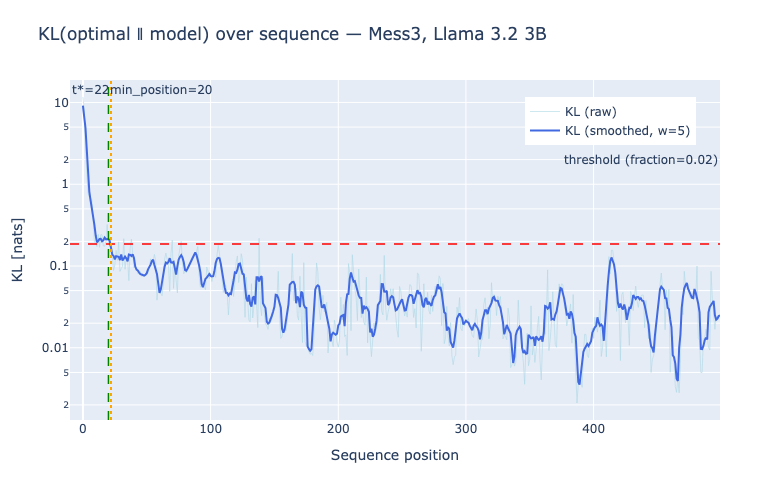
\includegraphics[width=0.72\textwidth]{figures/kl_over_sequence.png}
  \caption{KL divergence between the model's renormalized output distribution and the Bayesian-optimal distribution over the first 100 tokens of a Mess3 sequence. The dashed line indicates the convergence threshold (2\% of maximum KL). The model consistently reaches this threshold by around 20--30 tokens.}
  \label{fig:kl_over_sequence}
\end{figure}

\subsection{Linear decodability of belief states}

\paragraph{Probe performance.}
Linear probes trained on pooled activations achieve high $R^2$ across most layers (Figure~\ref{fig:r2_per_layer}). Performance peaks at layers 2--4, where the eval $R^2$ reaches approximately 0.999 (MSE $\approx 1.8 \times 10^{-4}$). Layer 0 is notably worse ($R^2 \approx 0.988$), and performance degrades at the final layers, reaching $R^2 \approx 0.985$ at layer 27. All probes are evaluated on held-out sequences that were not seen during training; the small gap between train and eval performance indicates that the probes generalize well.

\begin{figure}[htbp]
  \centering
  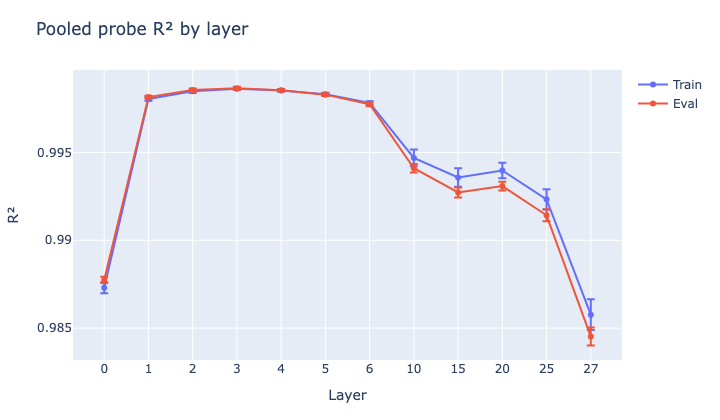
\includegraphics[width=0.72\textwidth]{figures/r2_per_layer.png}
  \caption{$R^2$ of the pooled linear probe evaluated on held-out sequences, by layer. Shading indicates one standard deviation across held-out sequences. Performance peaks in early-to-mid layers and is lower at the embedding layer (0) and at the final layers.}
  \label{fig:r2_per_layer}
\end{figure}

\paragraph{Cross-sequence consistency.}
Table~\ref{tab:cross_seq} reports pairwise probe similarity metrics across sequences at selected layers, using only post-convergence activations. At early layers, probes trained on different sequences recover nearly identical directions: at layer~0, the mean pairwise cosine similarity is 0.89 and the first principal angle $\theta_1$ is $23^\circ$, with a cross-MSE ratio near~1 (applying one sequence's probe to another's activations incurs almost no additional error). Probe directions diverge monotonically with depth: by layer~15, cosine similarity has dropped to 0.51 and $\theta_1$ has risen to $54^\circ$; by layer~27, cosine is 0.18 and $\theta_1$ reaches $75^\circ$ (near-orthogonal). The cross-MSE ratio peaks around layers 12--15 (${\sim}1.3$), where probes are still accurate individually but have diverged enough in direction that cross-application incurs meaningful additional error; at later layers the ratio decreases again because all probes, including self-evaluated ones, perform worse. This pattern indicates that the belief-state encoding is most canonical---shared across contexts---at the early layers where probe $R^2$ is also highest.

\begin{table}[htbp]
  \centering
  \caption{Pairwise similarity between per-sequence probes at selected layers. Cosine similarity and $\theta_1$ measure directional agreement between probe weight matrices; cross-MSE ratio measures the MSE penalty of applying one sequence's probe to another's activations.}
  \label{tab:cross_seq}
  \begin{tabular}{rccc}
    \hline
    Layer & Cosine sim.\ & $\theta_1$ (deg) & Cross-MSE ratio \\
    \hline
    0  & 0.89 & 22.9 & 1.00 \\
    3  & 0.70 & 36.6 & 1.07 \\
    10 & 0.64 & 46.7 & 1.24 \\
    15 & 0.51 & 53.9 & 1.32 \\
    25 & 0.33 & 62.8 & 1.22 \\
    27 & 0.18 & 74.5 & 1.09 \\
    \hline
  \end{tabular}
\end{table}

\paragraph{Emergence.}
Figure~\ref{fig:lag_summary} shows, for each layer, the mean lag between the token position at which the probe's $R^2$ crosses 0.9 and the token position at which the model's output KL converges. For layers 0--6, this lag is negative: for example, at layer 3, the probe threshold is reached approximately 6.3 tokens before the KL convergence point on average. At layer 10, the lag is approximately zero. At layers 15 and later, the probe trails the KL convergence by several tokens, reaching up to 26 tokens of lag at layer 27. This pattern is consistent with a computational pipeline in which the belief state is first assembled in a clean linear form at early layers, before the model's output distribution has converged, and is then transformed by later layers into a format that is less linearly decodable but more directly useful for output generation (see tuned lens results below). However, the lag at later layers may also partly reflect the lower cross-sequence consistency of those representations (Table~\ref{tab:cross_seq}): because the pooled probe's direction is a poorer match for any individual sequence at later layers, the $R^2$ threshold is reached later even if the information is present in a sequence-specific subspace.

\begin{figure}[htbp]
  \centering
  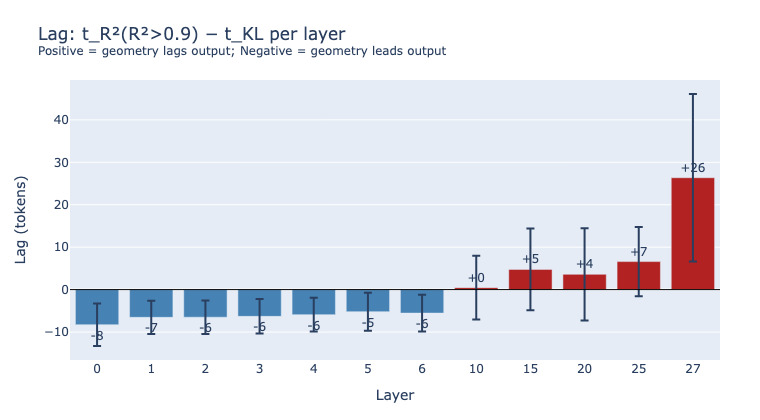
\includegraphics[width=0.72\textwidth]{figures/lag_summary.png}
  \caption{Mean lag (token position at which probe $R^2 > 0.9$ minus token position at which model KL converges) by layer. Negative values indicate that the probe threshold is reached before the model's output distribution converges. Error bars show one standard deviation across sequences.}
  \label{fig:lag_summary}
\end{figure}

The encoder-decoder results corroborate this picture: encoder $R^2$ is above 0.996 at layers 1--5, and degrades at later layers.

\paragraph{Belief geometry.}
Figure~\ref{fig:simplex} shows the belief states recovered by the encoder-decoder at layer 10, projected onto the 2-simplex. The recovered trajectories closely track the ground-truth belief state trajectory, and the distribution of points on the simplex reflects the stationary distribution of the Mess3 process.

\begin{figure}[htbp]
  \centering
  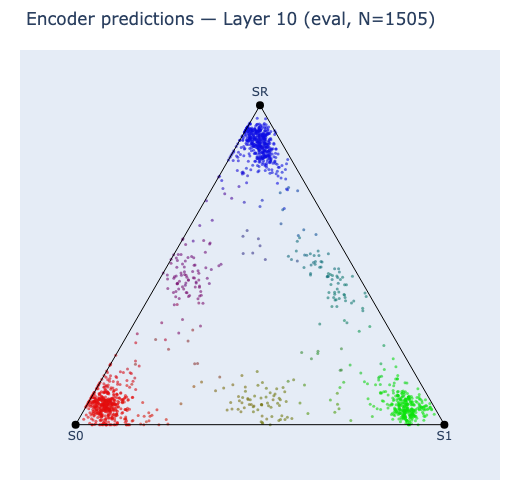
\includegraphics[width=0.55\textwidth]{figures/simplex_layer_10.png}
  \caption{Belief state geometry at layer 10 as recovered by the encoder-decoder. Each point represents the belief state at one token position, colored by the true hidden state. The distribution follows the expected shape of the Mess3 stationary distribution on the simplex.}
  \label{fig:simplex}
\end{figure}

\paragraph{Fern, Leopard, and belief-state sweep.}
We extend the belief-state probing analysis across 8 HMM configurations spanning three process families (Mess3, Fern, Leopard) with varying parameters. Table~\ref{tab:sweep_r2} summarizes the peak linear probe performance.

\begin{table}[htbp]
  \centering
  \caption{Peak belief-state probe $R^2$ across HMM configurations, with the layer at which the minimum KL(HMM $\|$ HMM-target tuned lens) is achieved.}
  \label{tab:sweep_r2}
  \begin{tabular}{lcccc}
    \hline
    Config & Best $R^2$ layer & Best $R^2$ & Min KL(HMM $\|$ tuned\_hmm) & at layer \\
    \hline
    mess3 ($\alpha{=}0.6$, $x{=}0.15$) & 3 & 0.9998 & 0.000027 & 3 \\
    mess3 ($\alpha{=}0.2$, $x{=}0.15$) & 3 & 0.9997 & ${\approx}0$ & 1 \\
    mess3 ($\alpha{=}0.6$, $x{=}0.5$) & 4 & 0.9954 & 0.000107 & 3 \\
    mess3 ($\alpha{=}0.2$, $x{=}0.5$) & 3 & 0.9928 & 0.000023 & 3 \\
    fern ($x{=}0.63$) & 5 & 0.9928 & 0.000097 & 5 \\
    fern ($x{=}0.4$) & 5 & 0.9757 & 0.000059 & 4 \\
    leopard ($x{=}0.15$) & 7 & 0.5727 & 0.031580 & 7 \\
    leopard ($x{=}0.5$) & 5 & 0.3337 & 0.009651 & 6 \\
    \hline
  \end{tabular}
\end{table}

The Fern results provide the strongest evidence that the model tracks genuine latent structure: despite the non-injective emission matrix (2 tokens, 3 states), linear probes achieve $R^2 > 0.97$ at layers 3--5, and the HMM-target tuned lens achieves KL $< 0.0001$. The model encodes a full 3D belief-state geometry even though its output distribution is one-dimensional, ruling out the hypothesis that the representation merely compresses output probabilities.

The Leopard process, by contrast, shows substantially weaker belief-state encoding ($R^2 \approx 0.33$--$0.57$). This is not simply a consequence of having two output tokens; Fern also has two tokens but achieves near-perfect $R^2$. The difference likely reflects Leopard's sparser, more deterministic transition structure, which may not align well with the model's inductive biases for in-context sequence prediction.

Figure~\ref{fig:pca_sweep} shows 2D PCA projections of residual stream activations for three representative configurations. For Mess3, the belief simplex is clearly visible in PC0--PC1 from early layers onward. For Fern, the geometry is discernible but occupies a smaller fraction of total activation variance. For Leopard, the belief structure is not visible in the top-2 principal components.

\begin{figure}[htbp]
  \centering
  \begin{minipage}[t]{0.32\textwidth}
    \centering
    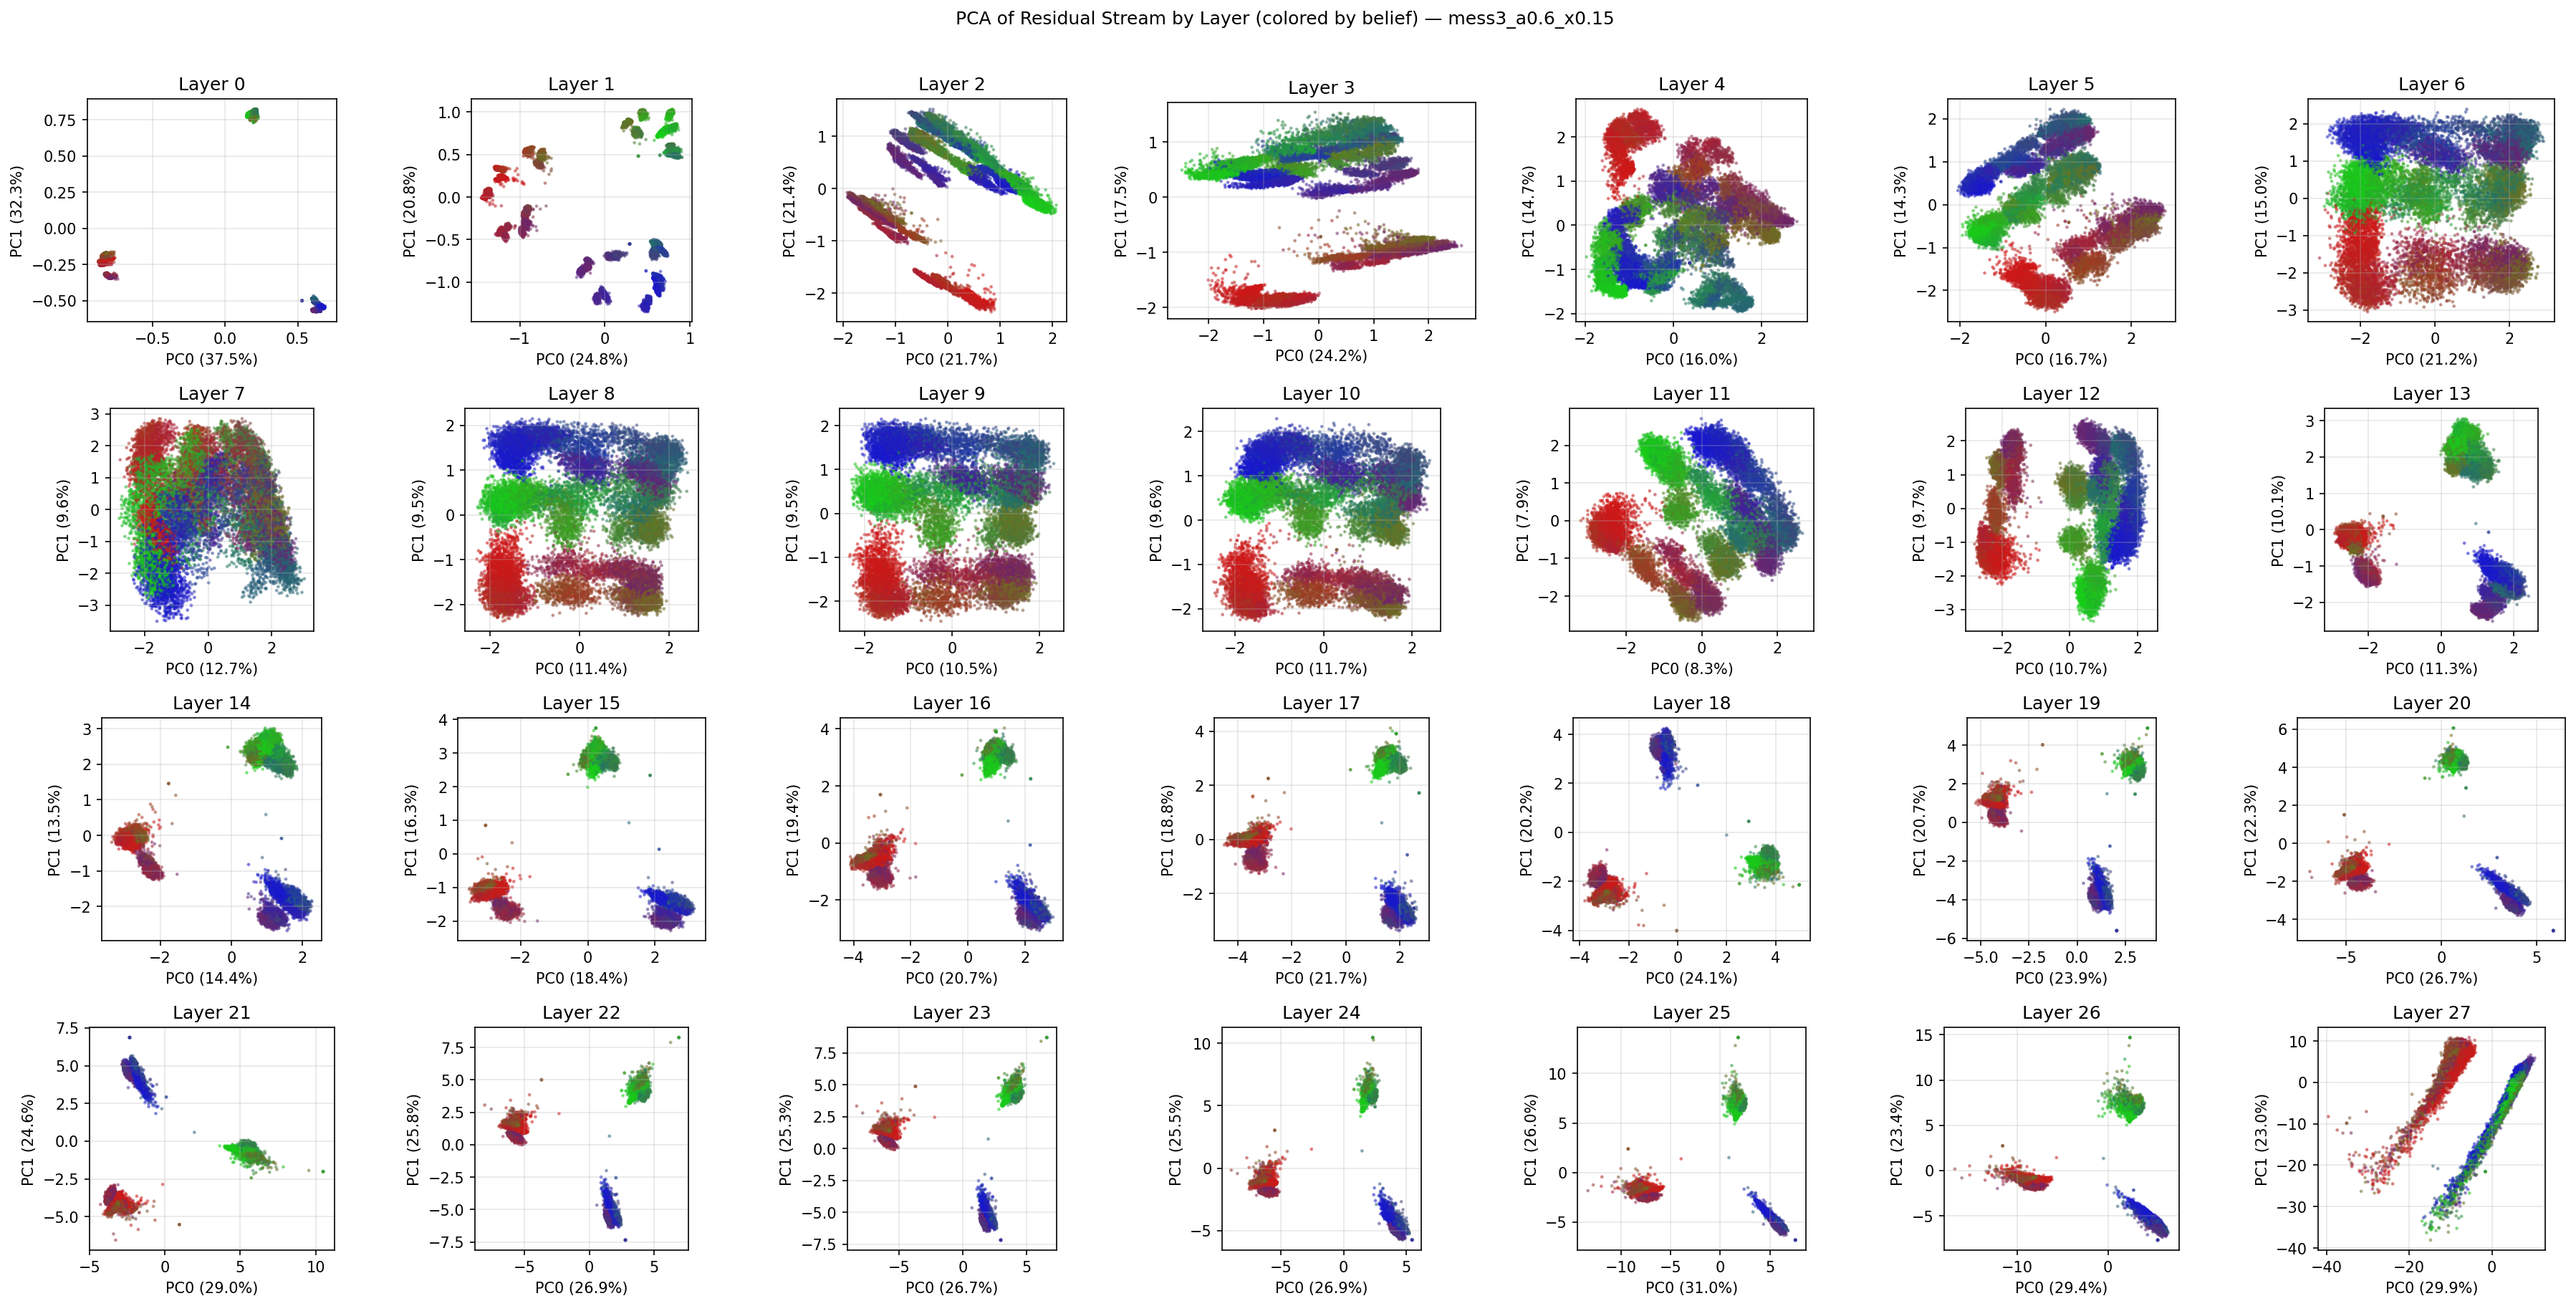
\includegraphics[width=\textwidth]{figures/pca_2d_mess3_a0.6_x0.15_midterm_report.png}
  \end{minipage}
  \hfill
  \begin{minipage}[t]{0.32\textwidth}
    \centering
    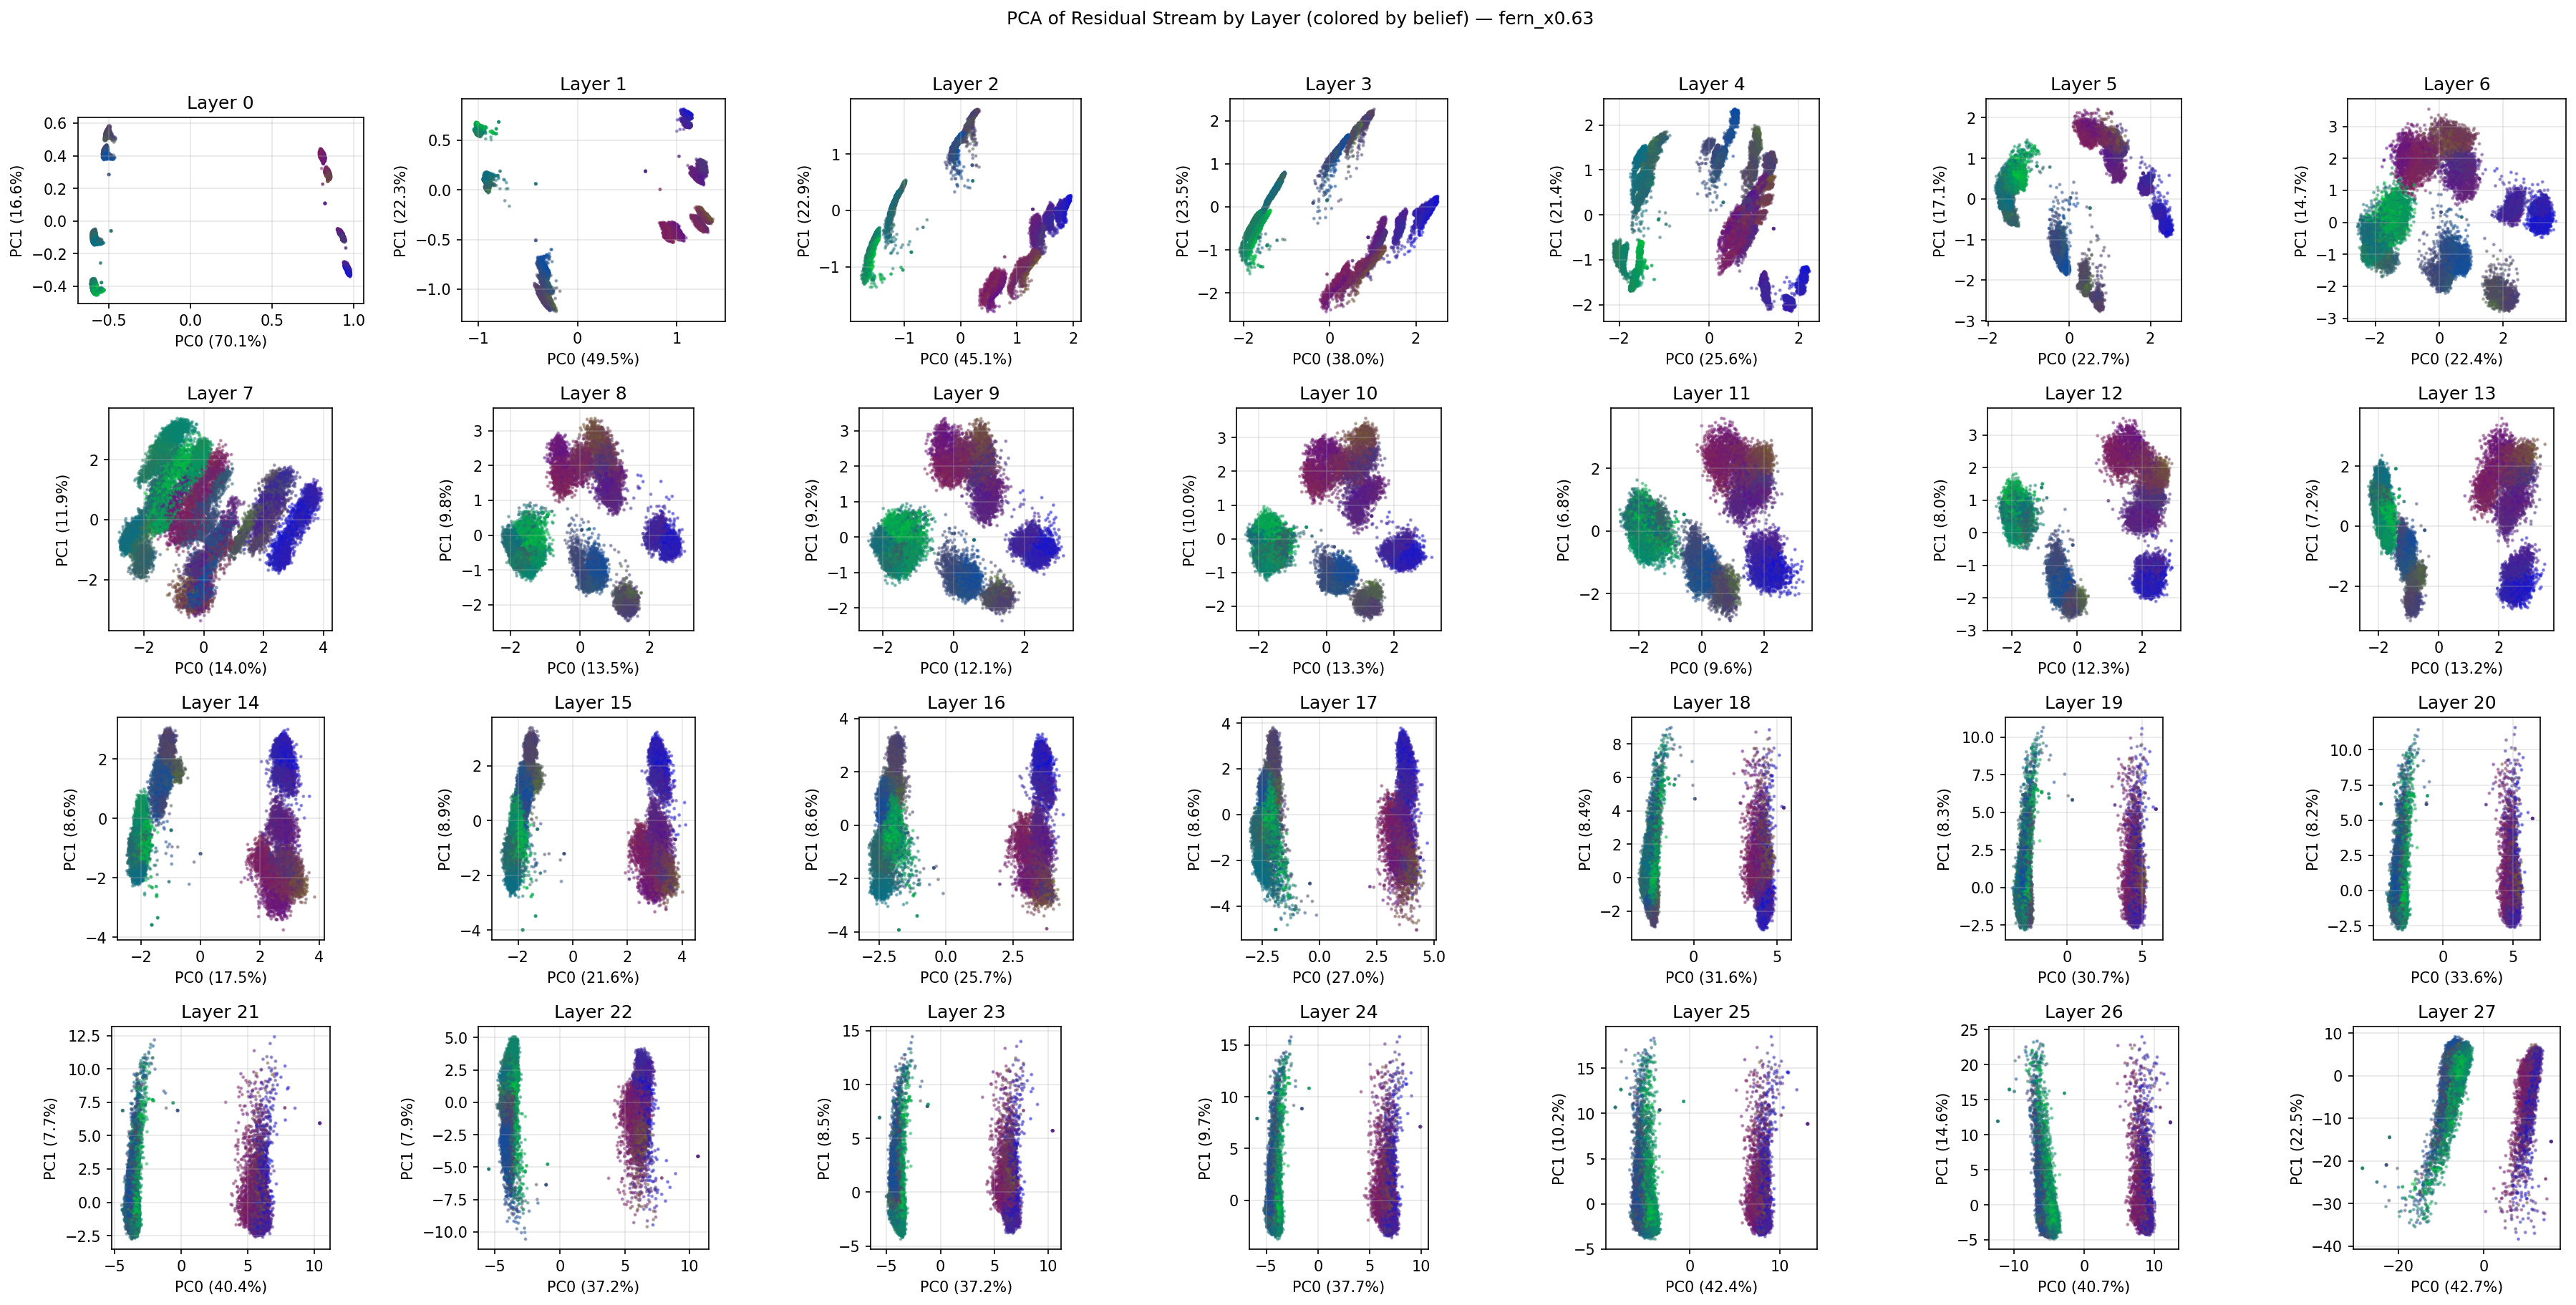
\includegraphics[width=\textwidth]{figures/pca_2d_fern_x0.63_midterm_report.png}
  \end{minipage}
  \hfill
  \begin{minipage}[t]{0.32\textwidth}
    \centering
    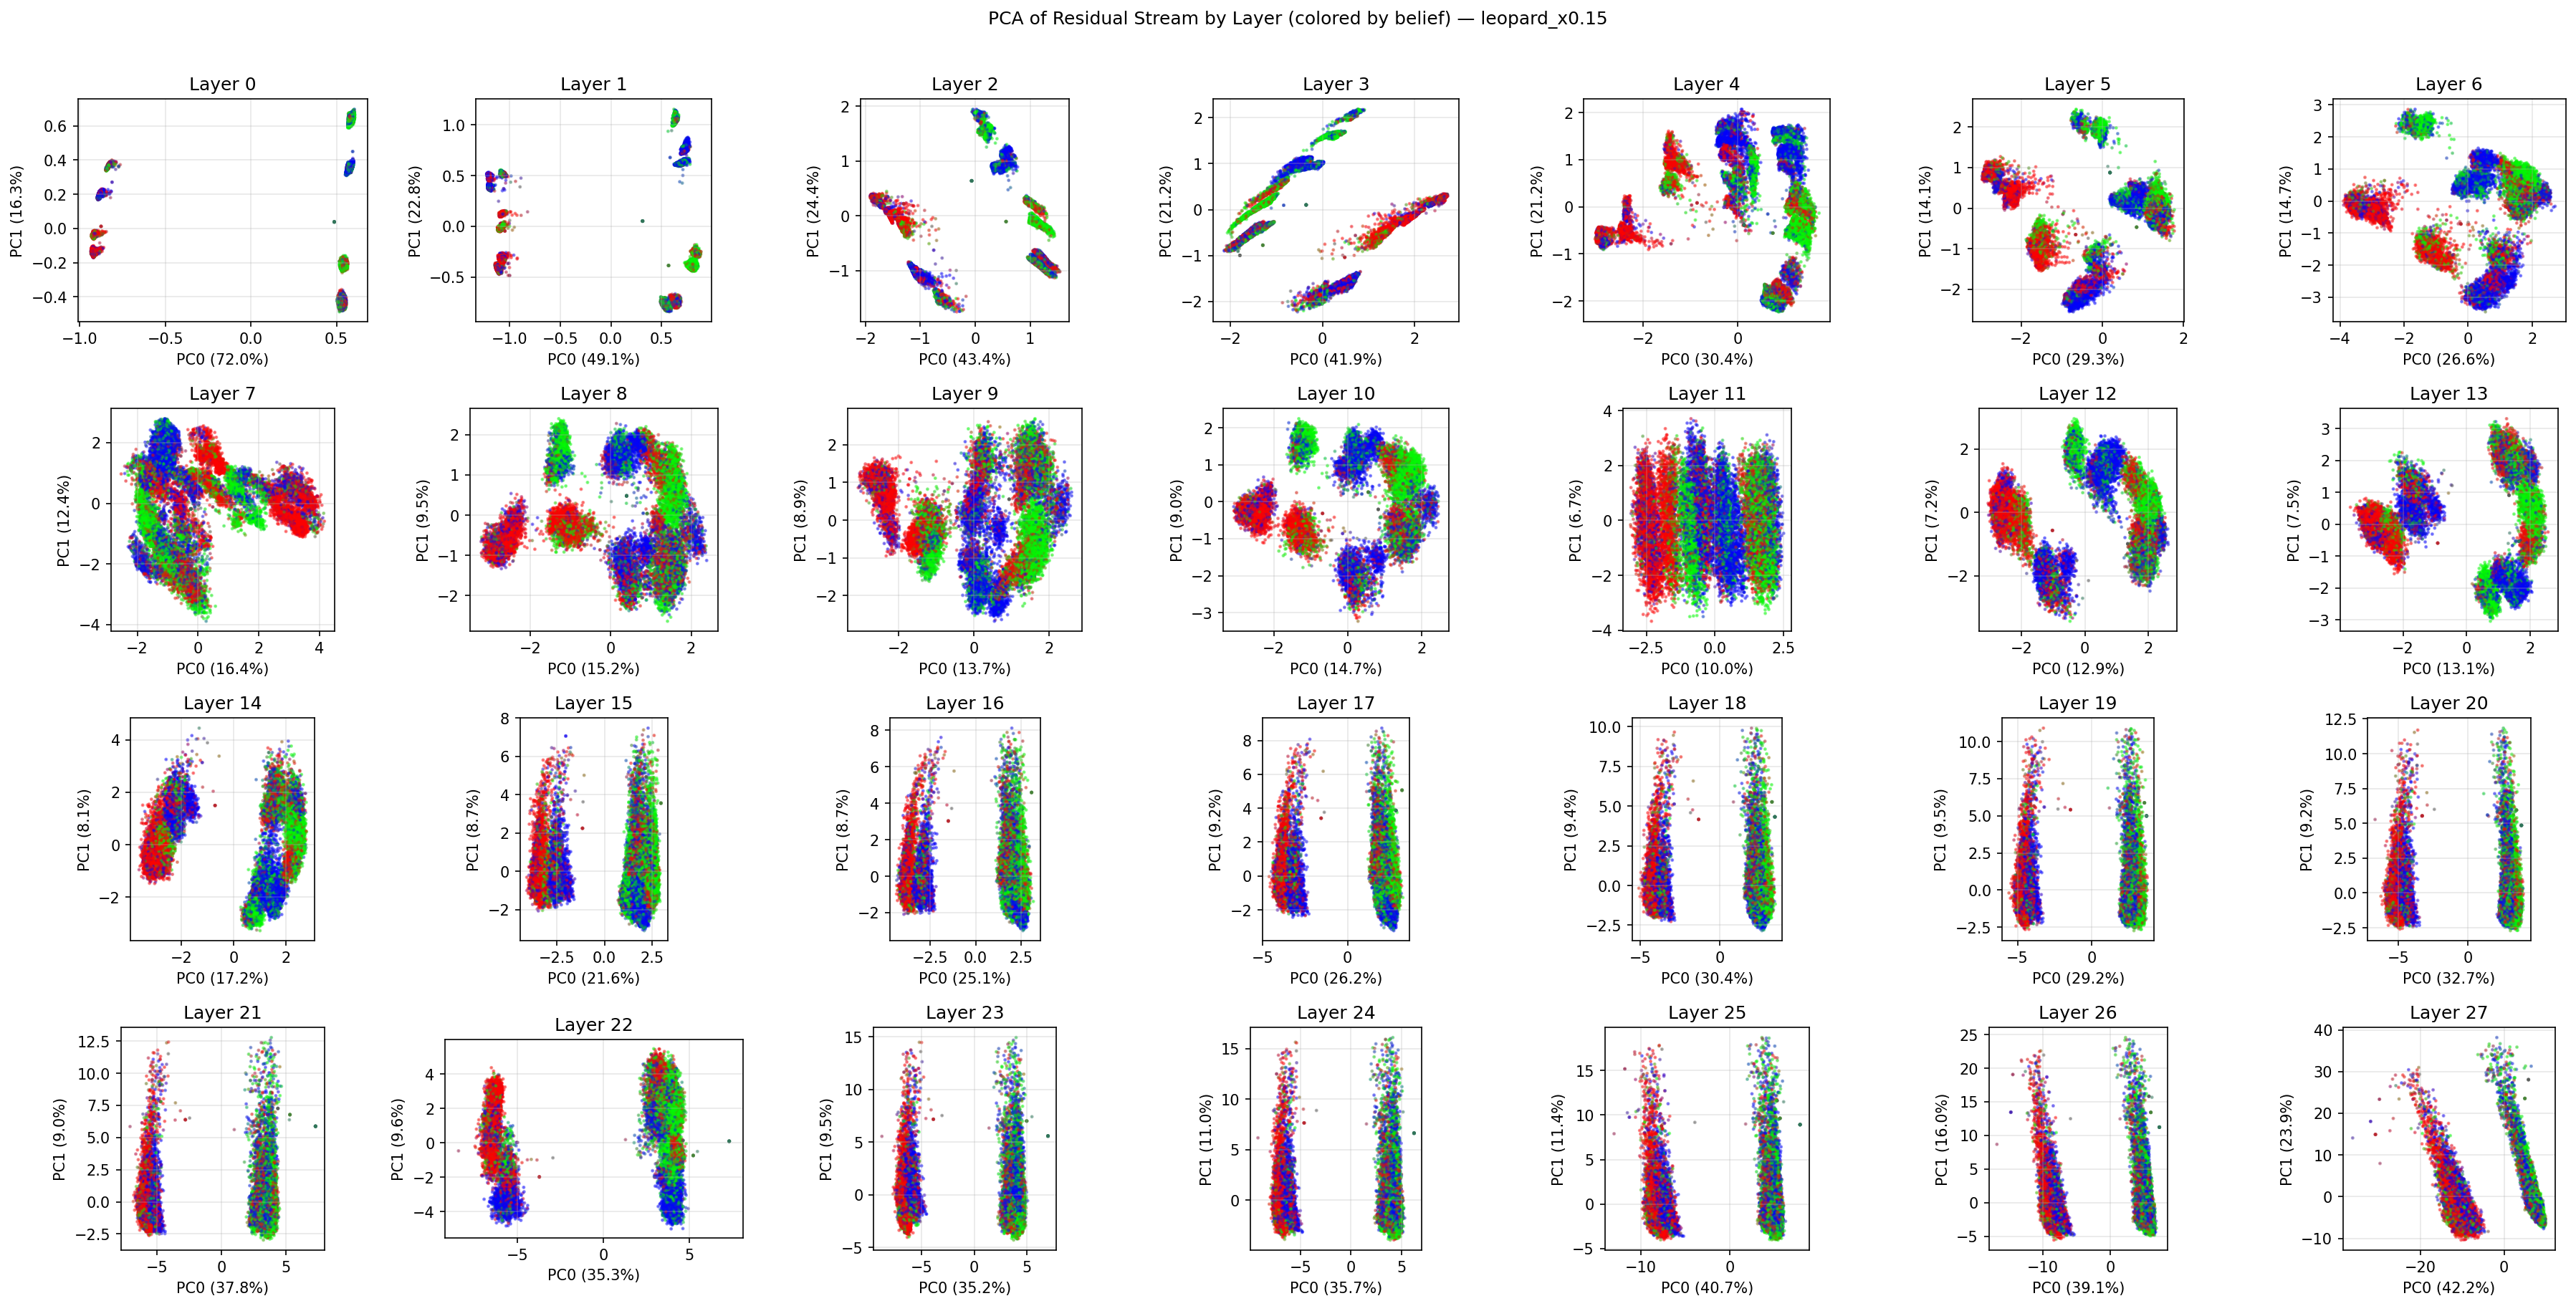
\includegraphics[width=\textwidth]{figures/pca_2d_leopard_x0.15_midterm_report.png}
  \end{minipage}
  \caption{2D PCA of residual stream activations across all 28 layers, colored by ground-truth belief state (RGB = $(b^{(1)}, b^{(2)}, b^{(3)})$). Left: Mess3 ($\alpha{=}0.6$, $x{=}0.15$) shows clear simplex geometry. Center: Fern ($x{=}0.63$) shows discernible but less crisp structure. Right: Leopard ($x{=}0.15$) shows no visible belief-state geometry in the top-2 PCA components.}
  \label{fig:pca_sweep}
\end{figure}

\paragraph{Tuned lens sweep.}
Figure~\ref{fig:tuned_lens_sweep} shows the layer-by-layer relationship between KL(HMM $\|$ HMM-target tuned lens) and belief-state probe $R^2$ across all 8 configurations. For Mess3 and Fern, the HMM-target tuned lens achieves near-zero KL ($< 0.001$) at the same early layers (3--7) where $R^2$ peaks, confirming that a simple affine transformation suffices to extract the belief state at these layers. The model-target tuned lens, by contrast, shows monotonically decreasing KL(model $\|$ tuned\_model) from layer 0 to 27, reflecting progressive convergence toward the final output distribution.

The cross-target comparison---KL(HMM $\|$ tuned\_model)---remains roughly constant across layers ($\sim$0.01--0.02), indicating that the model's internal predictions maintain a consistent gap from the HMM ground truth regardless of layer depth. This gap is process-dependent and correlates with the $R^2$ pattern: smaller for Mess3 and Fern, larger for Leopard.

\begin{figure}[htbp]
  \centering
  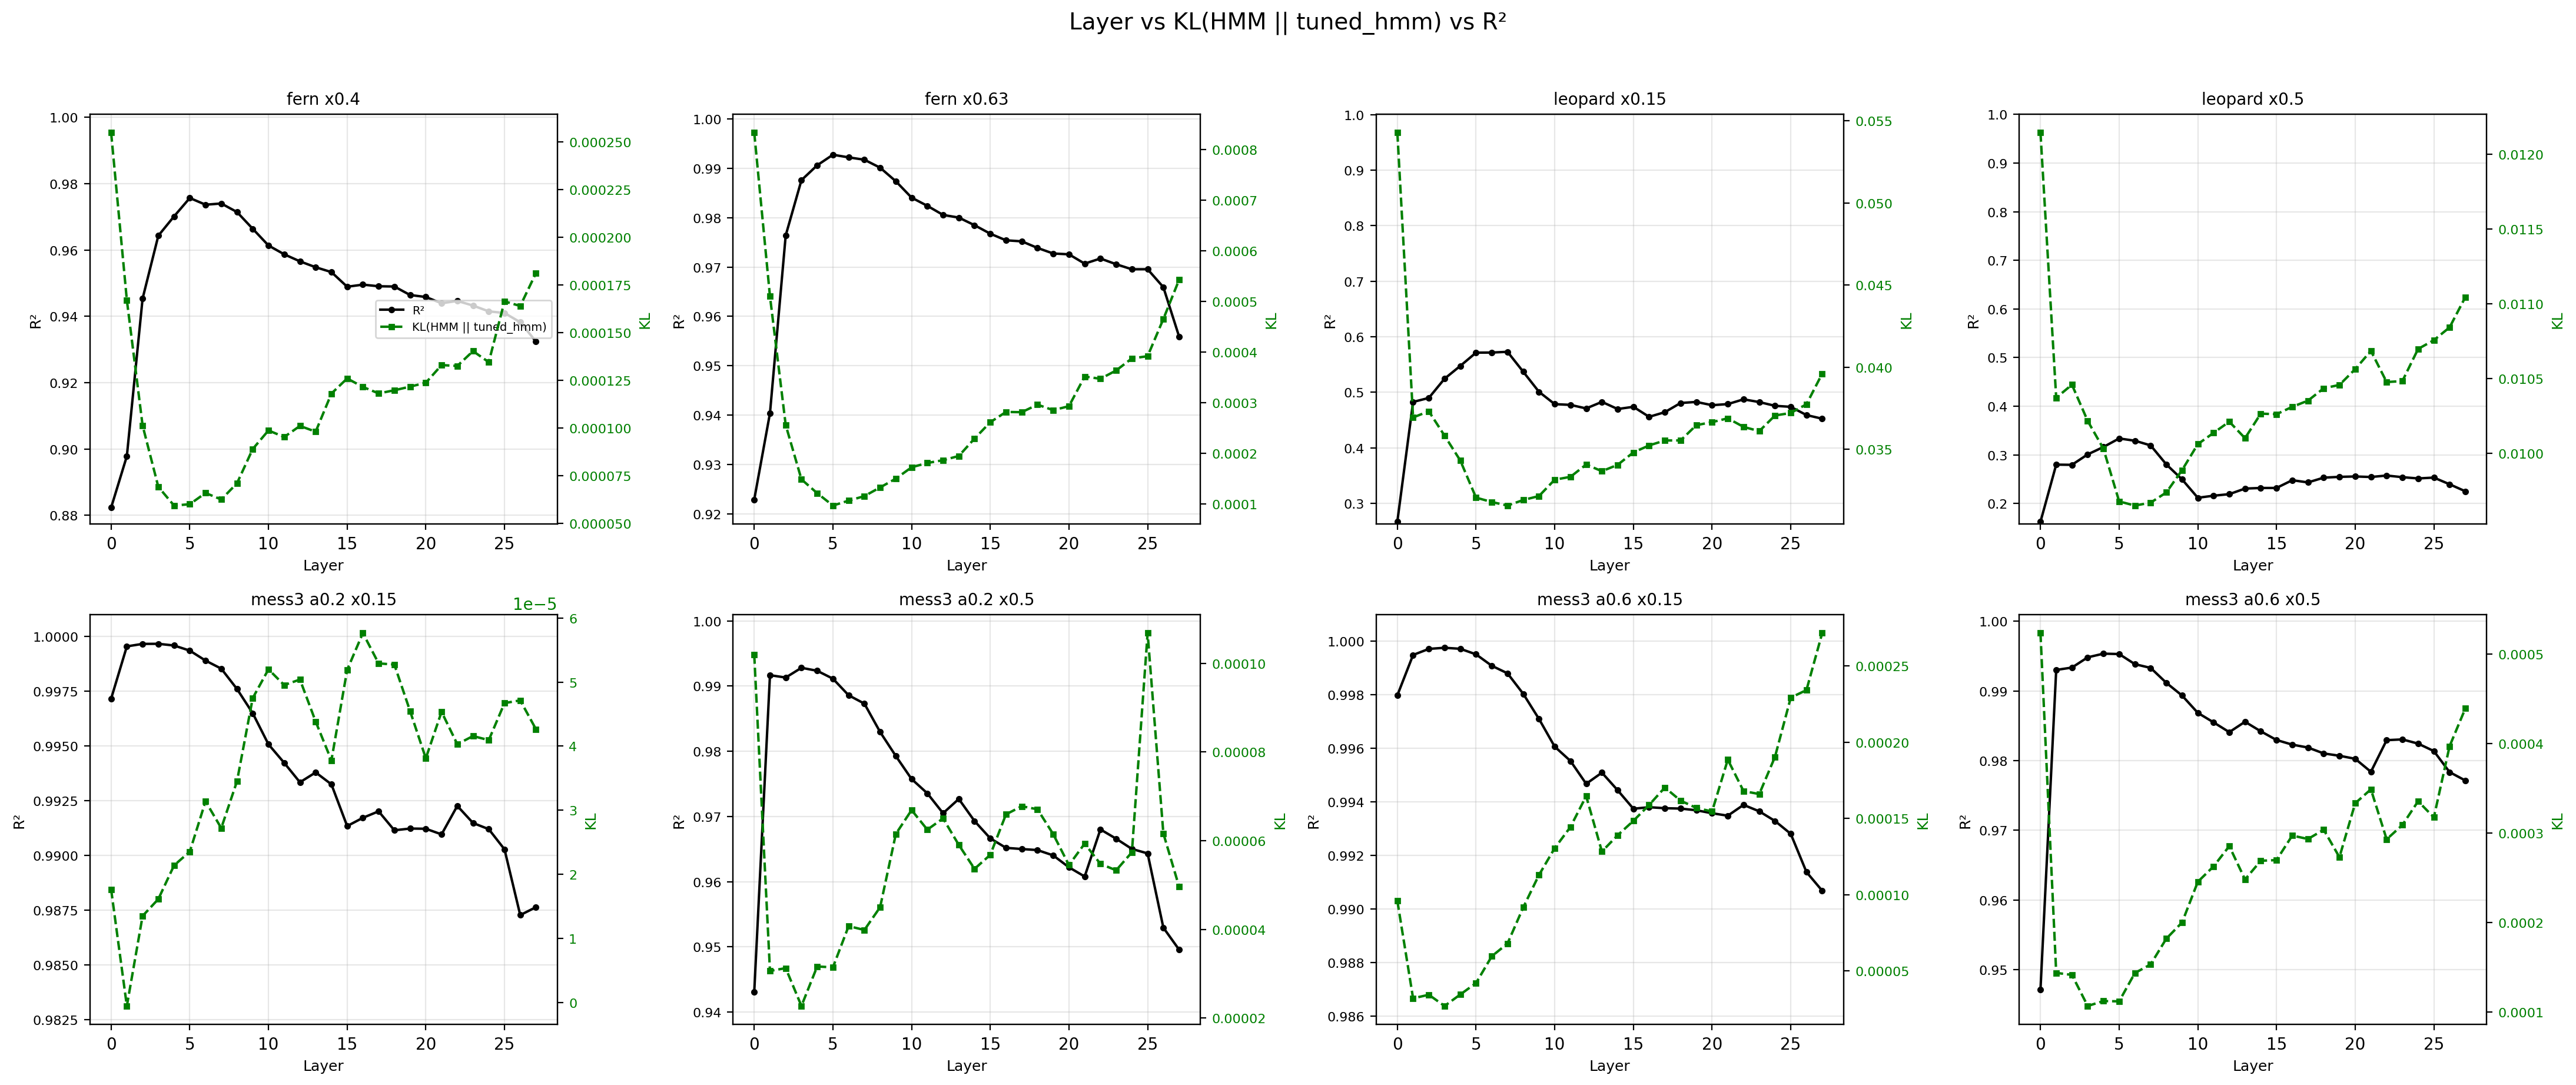
\includegraphics[width=\textwidth]{figures/layer_kl_hmm_tuned_hmm_vs_r2_midterm_report.png}
  \caption{Layer vs.\ KL(HMM $\|$ HMM-target tuned lens) vs.\ $R^2$ for all 8 HMM configurations. Black line (left axis): belief-state probe $R^2$. Colored dashed line (right axis): KL divergence. Mess3 and Fern achieve near-zero KL at the early layers where $R^2$ peaks; Leopard shows persistently higher KL.}
  \label{fig:tuned_lens_sweep}
\end{figure}

\subsection{Causal use of belief states}

\paragraph{Activation patching.}
In the unpatched baseline, the model's output distribution is close to the factual Bayesian-optimal predictions (mean KL = 0.030, $\sigma = 0.035$) and substantially further from the counterfactual (mean KL = 0.397, $\sigma = 0.166$). Figure~\ref{fig:crossing} shows the crossing plot: as the patching layer increases, the model's KL to the counterfactual decreases and its KL to the factual increases, consistent with the patched activations carrying information that shifts the model's beliefs toward the counterfactual. The effect is concentrated in the early-to-mid layers, broadly consistent with the probe results.

\begin{figure}[htbp]
  \centering
  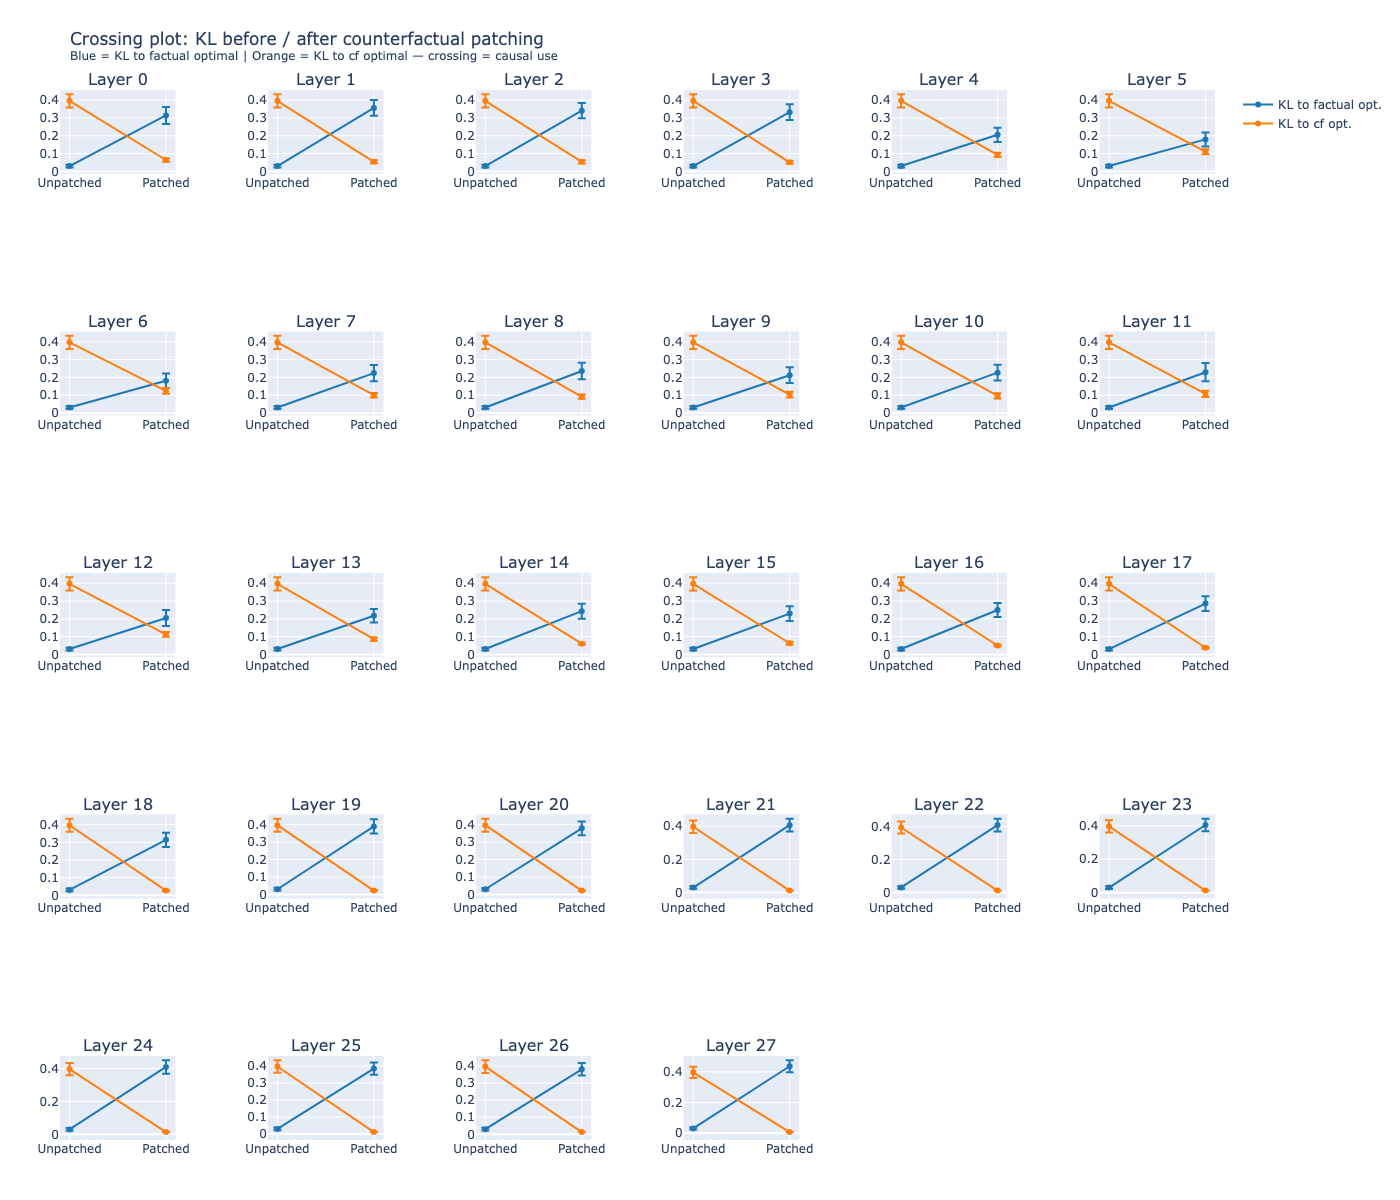
\includegraphics[width=0.72\textwidth]{figures/crossing_plot.png}
  \caption{Crossing plot for activation patching. The $y$-axis shows mean KL divergence to the factual (blue) and counterfactual (orange) Bayesian-optimal distributions, as a function of the layer at which patching is applied. The crossover point indicates the layer at which the patched activations carry sufficient belief state information to shift the model's predictions toward the counterfactual.}
  \label{fig:crossing}
\end{figure}

\paragraph{Factual--counterfactual discrepancy and token probability.}
Although the factual and counterfactual conditions share an identical prefix and differ only in the final token, counterfactual patches consistently yield higher KL to their target than factual patches. This is initially surprising, since attention at the intervention position draws on the same context in both cases.

To investigate, we designed a control experiment that crosses two binary factors: whether the patch is \emph{factual} (the variant sequence ends in the token whose belief is being injected) or \emph{counterfactual} (it ends in a different token), and whether the injected belief corresponds to a \emph{likely} or \emph{unlikely} next token under the prefix belief. For each base sequence, we generate all three variant sequences (one per possible final token) and all three target beliefs, yielding nine patch specs per sequence. A sanity check confirms that for a fixed target belief, patching KL is invariant across the three variant sequences (mean within-group standard deviation $\approx 0$), validating that causal masking isolates the intervention from the identity of the actual final token.

The main finding is that the factual--counterfactual distinction does not explain the KL gap. When we condition on token probability, the factual and counterfactual curves collapse: likely-token beliefs are reconstructed well regardless of whether the patch is factual or counterfactual, while unlikely-token beliefs show higher KL in both cases (Figure~\ref{fig:patching_token_prob}). The apparent factual advantage arises because, under the Mess3 parameterization, one token is typically much more probable than the other two at any given state, so factual patches disproportionately correspond to likely tokens.

\begin{figure}[htbp]
  \centering
  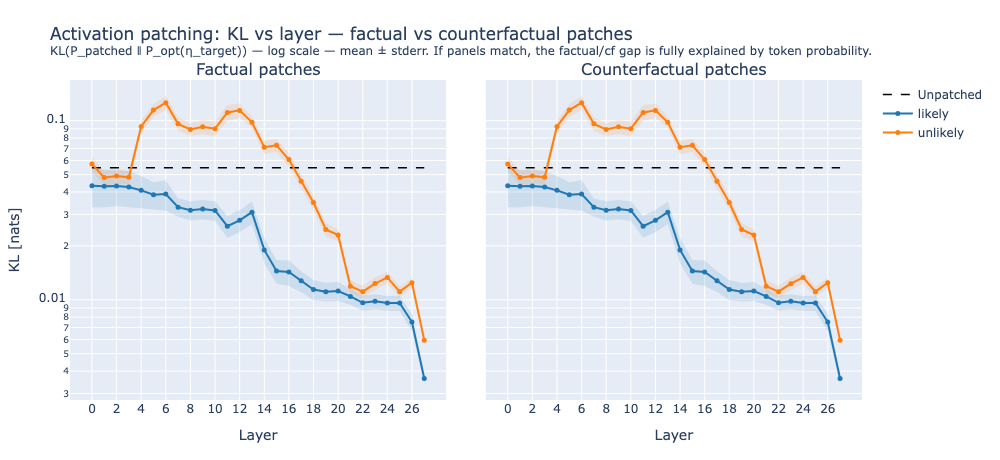
\includegraphics[width=0.82\textwidth]{figures/patching_token_prob.png}
  \caption{Activation patching KL vs.\ layer, split by token probability. Left: factual patches; right: counterfactual patches. In both panels, likely-token beliefs (blue) yield lower KL than unlikely-token beliefs (orange). The two panels are nearly identical, confirming that the factual--counterfactual distinction is not the relevant factor; token probability is.}
  \label{fig:patching_token_prob}
\end{figure}

\paragraph{Decoder fidelity.}
To confirm that the probability effect originates in the decoder rather than in the model's downstream computation, we measure decoder reconstruction error as a function of token probability $p_t = P(x_t \mid \mathbf{b}_{t-1})$. For each sequence position after a transient cutoff, we compute both the decoder-only MSE $\lVert \mathbf{a}_t - D(\mathbf{b}_t) \rVert^2$ (comparing the actual activation to the decoder's output given the true belief) and a round-trip MSE $\lVert \mathbf{a}_t - D(E(\mathbf{a}_t)) \rVert^2$ (encoding the activation and decoding it back). Both metrics show a negative correlation with $p_t$: belief states associated with unlikely tokens have systematically higher reconstruction error, particularly at early-to-mid layers where the patching effect is strongest (Figure~\ref{fig:decoder_fidelity}). This confirms that the decoders, trained on the natural distribution of Mess3 activations, are less faithful for beliefs corresponding to rare emissions---precisely the regime that dominates counterfactual patches.

\begin{figure}[htbp]
  \centering
  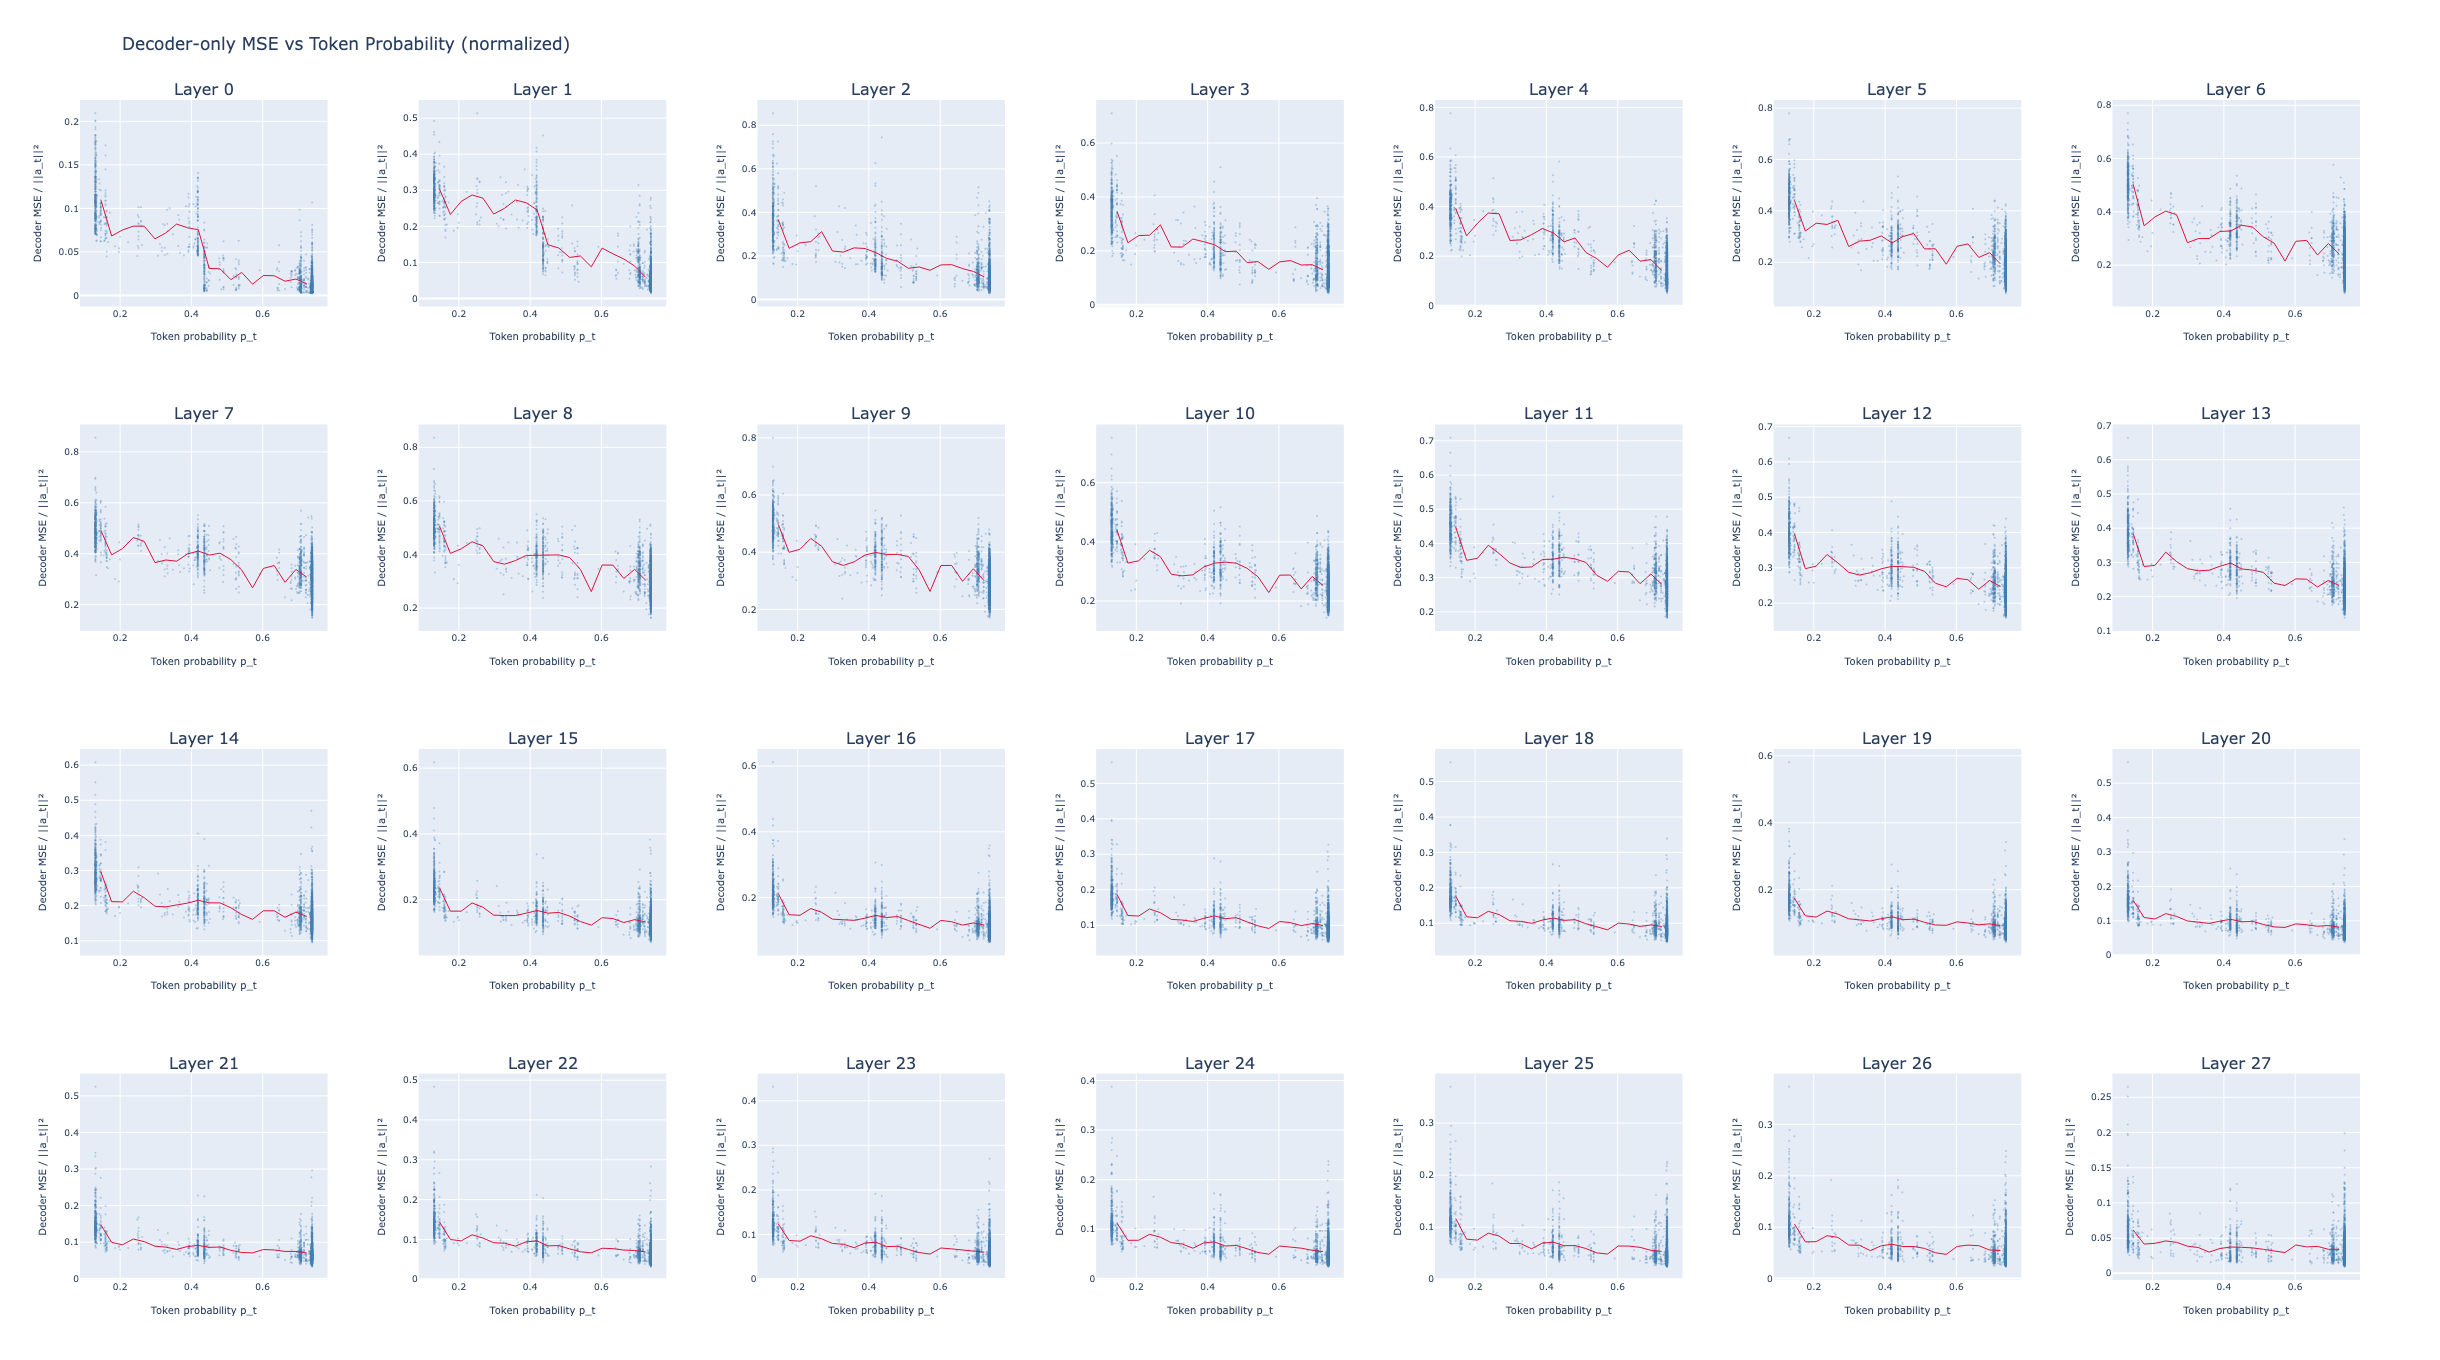
\includegraphics[width=0.95\textwidth]{figures/decoder_fidelity.png}
  \caption{Normalized decoder MSE ($\lVert \mathbf{a}_t - D(\mathbf{b}_t) \rVert^2 / \lVert \mathbf{a}_t \rVert^2$) vs.\ token probability $p_t$ at each layer. Each blue dot is one (sequence, position) pair; the red line shows the binned mean. At early-to-mid layers, low-probability tokens exhibit markedly higher reconstruction error, explaining why patching with beliefs corresponding to unlikely tokens yields worse results.}
  \label{fig:decoder_fidelity}
\end{figure}

\paragraph{Activation steering.}
Steering successfully shifts the model's output distribution toward the target belief state across all conditions. Figure~\ref{fig:steering_kl} shows KL divergence to the target as a function of the intervention layer. In the unsteered baseline the model's output is already close to its factual optimum (mean KL~$= 0.029$, $\sigma = 0.031$); steering drives the output toward a \emph{different} target belief, and the KL to that target drops to comparable levels at the best-performing layers.

For the past-consistent conditions, steering at late layers (21--27) achieves KL to target below 0.03 for all tested values of $K$, approaching the unsteered baseline level. At the early-to-mid layers where linear probes are strongest (layers 2--4), steering also performs well: for $K = 1$, KL to target at layer~3 is $0.045 \pm 0.037$. Steering at middle layers (5--13) shows somewhat higher KL, consistent with the pattern seen in patching.

The shared-prefix and different-prefix variants of the past-consistent condition yield broadly similar KL-to-target curves across layers and $K$ values, with no systematic advantage for either variant. This suggests that prefix-attention conflict---where the source prefix is inconsistent with the injected donor trajectory---does not substantially degrade steering performance, and the belief-injection effect is the dominant factor.

The control conditions confirm the specificity of the intervention. Garbage-valid steering (target is a real Mess3 belief from an unrelated sequence) achieves KL to target of $0.136 \pm 0.096$ at layer~3, substantially worse than past-consistent steering at the same layer, but still converges to near-baseline levels at late layers. Garbage-random steering (target sampled uniformly from the simplex) follows a similar pattern, with consistently higher KL than the garbage-valid condition at early and mid layers.

These steering results were obtained with the same decoders used in the patching experiments, before the decoder fidelity issue described above was identified. The elevated KL at middle layers (roughly 6--17) may therefore reflect the same decoder bias toward likely-token beliefs rather than a genuine limitation of the steering intervention. Whether this mid-layer KL gap persists once decoders are retrained on a probability-balanced dataset remains to be tested.

\begin{figure}[htbp]
  \centering
  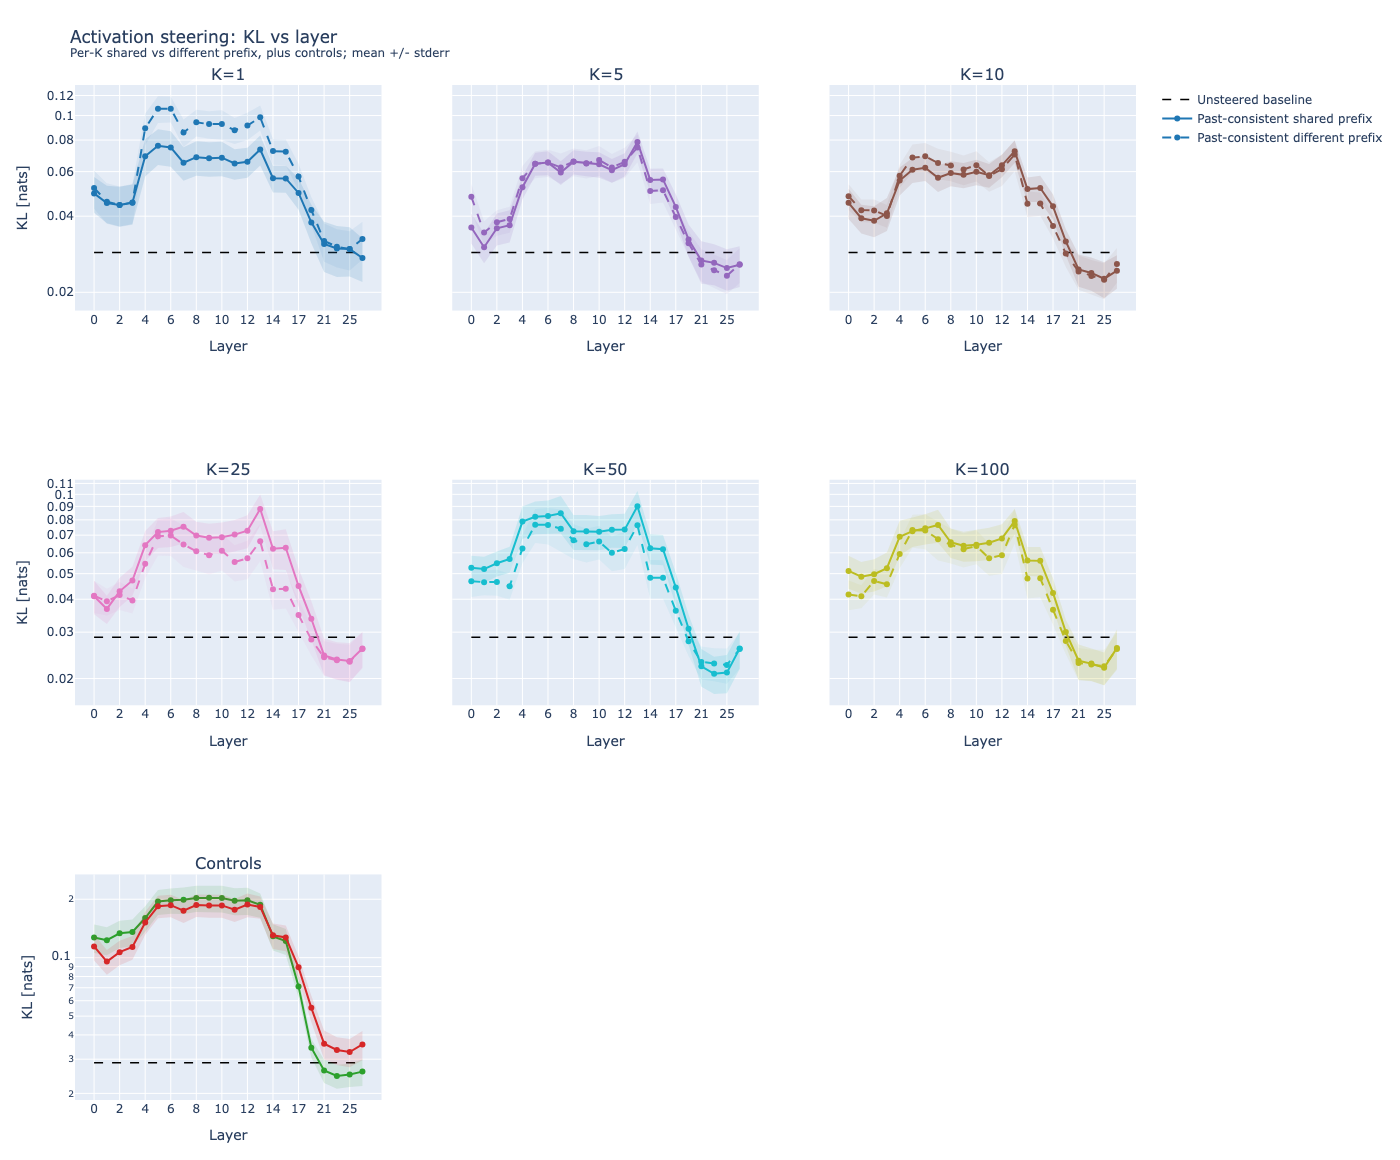
\includegraphics[width=\textwidth]{figures/steering_kl_vs_layer.png}
  \caption{Activation steering: KL divergence to the target belief state as a function of intervention layer, for past-consistent conditions at each $K$ (top two rows) and control conditions (bottom). Solid lines show the shared-prefix variant; dashed lines show the different-prefix variant. The black dashed line indicates the unsteered baseline KL (to the factual belief). At late layers, all conditions converge to near-baseline KL, indicating successful belief injection.}
  \label{fig:steering_kl}
\end{figure}

\paragraph{Tuned lens.}
The model-target tuned lens reveals a sharp improvement in per-layer predictions beginning around layers 13--14, after which KL divergence to the Bayesian-optimal distribution drops substantially. Strikingly, this improvement occurs precisely in the layers where linear probe $R^2$ is \emph{lower} than its early-layer peak (Figure~\ref{fig:r2_per_layer}). Early layers (2--4), where linear probes achieve their highest $R^2$, do not yield correspondingly better model-target tuned lens decoding. This dissociation suggests that the quality of the linear belief-state encoding is not the primary determinant of whether a layer's activations are sufficient to recover the correct output distribution.

However, the \emph{HMM-target} tuned lens tells a complementary story: when the translator is trained to decode toward the HMM's observation probabilities rather than the model's own output, KL(HMM $\|$ tuned\_hmm) is minimized at precisely the early layers (3--7) where probe $R^2$ peaks. This confirms that the belief state is most faithfully encoded at early layers; the model-target tuned lens's late-layer improvement instead reflects the accumulation of output-formatting computation that is orthogonal to the belief geometry. The later-layer computation analysis (Section~\ref{sec:later_layer}) corroborates this interpretation.

\paragraph{Later-layer computation.}
\label{sec:later_layer}
Decomposing activations into belief-aligned and orthogonal components reveals that belief-state variance decreases monotonically from $\sim$1--4\% at layer 0 to $\sim$0.1--0.2\% at layer 27, while orthogonal variance grows correspondingly. Yet decoders trained on the \emph{full} activation vector improve with depth ($R^2$: 0.955 at layer 0 $\to$ 0.984 at layer 27), while decoders restricted to the belief subspace remain poor ($R^2 \approx 0.2$). This means later layers encode prediction-relevant information \emph{orthogonal} to the belief subspace---performing output formatting and logit refinement rather than improving the belief representation itself. This ``compute early, format late'' pattern is consistent across Mess3 and Fern configurations.

\subsection{Construction of belief states}

\textit{Andrew to add.}

% ============================================================================
% CHALLENGES & OPEN QUESTIONS
% ============================================================================
\section{Challenges \& Open Questions}

The Fern results substantially resolve the ambiguity between genuine latent-state tracking and linear encoding of the output distribution. Fern's emission matrix maps three hidden states to two output tokens without a left inverse, so the output distribution does not uniquely determine the belief state. Despite this, linear probes recover the full 3D belief state with $R^2 > 0.97$, and the HMM-target tuned lens achieves KL $< 0.0001$ at early layers. This rules out the hypothesis that the model merely compresses its output probabilities, and provides strong evidence that Llama-3.2-3B tracks genuine latent structure when processing HMM-generated sequences.

The belief-state sweep across Mess3, Fern, and Leopard reveals that the model's ability to encode belief states varies substantially by process. Mess3 and Fern achieve near-perfect encoding ($R^2 > 0.97$), while Leopard is poorly captured ($R^2 \approx 0.33$--$0.57$). Understanding what structural properties of the HMM determine encoding quality---transition matrix sparsity, mixing time, emission geometry---remains an open question.

On the causal side, the patching experiments demonstrate that activations carry belief state information, but the decoder fidelity analysis reveals that the decoders used to construct the intervention are systematically less accurate for belief states corresponding to unlikely tokens. Because Mess3 concentrates probability mass on one token per state, the natural training distribution under-represents rare emissions, introducing a confound into any comparison that aggregates across token probabilities. Until this is addressed, intervention results for unlikely-token beliefs should be interpreted with caution.

Computationally, the belief-state sweep across 8 HMM configurations has been completed, revealing a clear hierarchy of encoding quality: Mess3 $>$ Fern $\gg$ Leopard. A Fern-specific challenge is that the 2-token vocabulary produces higher ``junk mass'' (probability assigned to non-HMM tokens) than the 3-token Mess3 vocabulary, which can inflate KL divergence metrics. Additionally, Leopard's poor encoding quality ($R^2 \approx 0.33$--$0.57$) raises the question of whether the model genuinely fails to track the Leopard belief state, or whether the belief state is encoded in a non-linear or higher-dimensional subspace not captured by our linear probes.

A further open question concerns an apparent tension between the tuned lens results and the probe and intervention results. The belief-state geometry is cleanest in early layers: linear probes peak at layers 2--4, cross-sequence consistency is highest there, and the belief-state representation emerges before the model's output distribution has converged. Yet tuned lens decoding performs \emph{worst} at precisely these early layers and only achieves low KL divergence after a sharp improvement around layers 13--14. The causal experiments echo this pattern: activation patching and steering are most effective at late layers (roughly 14+), where the linear belief-state encoding is weaker. This is counter-intuitive: the layers where the belief geometry is most linearly decodable are the layers where it is hardest to find a map from that geometry to the output probabilities, whereas the layers where the geometry is dirtier are the layers where causal interventions and tuned lens decoding are most effective. Several hypotheses could explain this: (a) the linear belief-state representation is progressively transformed by later attention and MLP layers into a format optimized for output generation rather than linear readout, (b) later layers contain information about the sequence that is relevant to prediction but not captured by the belief-state geometry, or (c) the degradation of the linear encoding in later layers is compensated by other computational mechanisms. Ablation experiments---projecting out the linear belief-state subspace at various layers and measuring the downstream effect on tuned lens performance---would help distinguish these hypotheses.

% ============================================================================
% NEXT STEPS
% ============================================================================
\section{Next Steps}

The belief-state sweep and tuned lens sweep experiments are complete across 8 HMM configurations (4 Mess3, 2 Fern, 2 Leopard). The key finding is that belief-state encoding quality varies substantially by process, with Mess3 and Fern achieving near-perfect linear decodability ($R^2 > 0.97$) while Leopard is poorly captured ($R^2 \approx 0.33$--$0.57$). The Fern results are particularly important: they demonstrate genuine latent-state tracking (not just output compression) by showing that the model encodes a 3D belief state from a 1D output distribution. The tuned lens sweep confirms that the optimal decoding window is at early layers (3--7) across all well-encoded processes, and that later layers perform output formatting rather than belief refinement. Remaining work includes extending the activation patching and steering pipeline to Fern and Leopard to test whether the causal findings from Mess3 generalize, and investigating whether non-linear probes can recover the Leopard belief state that linear probes miss.

For the causal interventions, the most immediate priority is to retrain the decoders on a dataset of activations that is balanced with respect to token probability. Because Mess3 concentrates most emissions on a single likely token per state, the natural distribution of training activations under-represents rare emissions, leading to higher decoder reconstruction error for unlikely-token beliefs. By subsampling token positions to equalize the representation of likely and unlikely emissions, we aim to flatten the decoder MSE across the probability range and thereby remove the confound from all downstream patching and steering experiments. Additionally, the steering experiments are partially complete but need further analysis and comparison across layers and $k$ values.

Resolving the tension between the probe, tuned lens, and intervention layer profiles is a central priority. The belief-state geometry is cleanest where tuned lens decoding and causal interventions are weakest, and vice versa. Understanding what computational mechanisms in later layers enable effective output prediction despite a weaker linear belief-state encoding is essential. Ablation experiments that selectively remove the belief-state subspace from residual stream activations at various layers are a natural candidate; if the tuned lens performance at later layers survives ablation of the belief-state subspace, this would indicate that later layers rely on information beyond the linear belief geometry.

A natural extension is to run similar experiments on other Simplexity processes with varying emission geometries, to understand what properties of the HMM determine whether and how the belief state is encoded. We may also consider running experiments on Llama-3.2-1B to study how model size affects the representations.

More broadly, the work so far has focused on three questions: (1) verifying that a production-scale LLM can predict HMM-generated data near-optimally in context, (2) establishing that the belief-state geometry is linearly present in the residual stream, and (3) demonstrating through causal interventions that this geometry is used by the model's downstream computation. A natural next direction is to shift focus toward understanding \emph{how} the belief geometry is formed: what mechanisms in the early layers give rise to it, how attention and MLP components contribute to constructing the belief state from context, and how the resulting representation is routed through later layers to the model's output. The investigation of constrained belief updates is a first step in this direction; extending this line of work to identify the specific circuits responsible for belief-state construction and routing would deepen our mechanistic understanding of in-context latent-state tracking.

% ============================================================================
% BIBLIOGRAPHY
% ============================================================================
\bibliographystyle{plain}
\bibliography{references}

\end{document}
